\documentclass[11pt,a4paper,twoside]{tesis}
% SI NO PENSAS IMPRIMIRLO EN FORMATO LIBRO PODES USAR
%\documentclass[11pt,a4paper]{tesis}

\usepackage{graphicx}
\usepackage[utf8]{inputenc}
\usepackage[spanish]{babel}
\usepackage[left=3cm,right=3cm,bottom=3.5cm,top=3.5cm]{geometry}

%%%%%%%%%%%%%%%%%%%%%%%%%%%%%%%%%%%%%%%%%%%%%%%

\usepackage[inline]{enumitem}									% control layout of itemize, enumerate, description
\usepackage{xspace}												% correct added/missing spaces made by tex decoder
\usepackage{pifont}												% for check and cross marks
\usepackage{mathtools}                                          % load amsmath, position eqs at fixed position,etc
\usepackage{amssymb}											% for extra symbols
%\usepackage{amsthm}											%for qed
\usepackage{trimclip}                                           % for cliping symbols in boxes
\usepackage[usenames,dvipsnames,svgnames,table]{xcolor}			% adds use of colors
\usepackage{listings}											% for the lstlisting environment
\usepackage{url}                                                % for url and hyperlinks

\usepackage[hidelinks]{hyperref}

\usepackage{subcaption}
\usepackage{placeins}

\bibliographystyle{plain}

%%%%%%%%%%%%%%%%%%%%%%%%%%%%%%%%%%%%%%%%%%%%%%%%%%%%%%%%%%%%%%%%%%%%%%%%%%%%%%%
%%  Modifiers and Fonts
%%%%%%%%%%%%%%%%%%%%%%%%%%%%%%%%%%%%%%%%%%%%%%%%%%%%%%%%%%%%%%%%%%%%%%%%%%%%%%%

\renewcommand{\k}[1]{\textit{#1}}
\newcommand{\mk}[1]{\mathit{#1}}

\renewcommand{\v}[1]{\texttt{#1}}
\newcommand{\mv}[1]{\text{\small\textsf{#1}}\xspace}
\newcommand{\mvs}[1]{\text{\scriptsize\textsf{#1}}\xspace}

\newcommand{\sref}[2]{\ref{#1}{\color{BrickRed}.}{\subref*{#1:#2}}}

%%%%%%%%%%%%%%%%%%%%%%%%%%%%%%%%%%%%%%%%%%%%%%%%%%%%%%%%%%%%%%%%%%%%%%%%%%%%%%%
%%  Symbols
%%%%%%%%%%%%%%%%%%%%%%%%%%%%%%%%%%%%%%%%%%%%%%%%%%%%%%%%%%%%%%%%%%%%%%%%%%%%%%%

% Tildes and crosses

\newcommand{\Y}{\ding{51}}
\newcommand{\N}{\ding{55}}

% Math

\newcommand{\card}[1]{\lvert#1\rvert}
\newcommand{\<}{\langle}
\renewcommand{\>}{\rangle}
\newcommand{\ldot}{\;.\;}
\newcommand{\lcom}{\,,\,}
\newcommand{\primeI}[1]{{#1}'}
\newcommand{\primeII}[1]{{#1}'\!\!\:'}
\newcommand{\into}{\mapsto}
\newcommand{\Nat}{\mathbb{N}}
\newcommand{\dotrightarrow}{\clipbox{0pt 0 {.675\width} 0}{\ensuremath{\rightarrow}} \makebox[1.1pt]{} {\cdot} {\cdot} {\cdot} \makebox[1.1pt]{} \clipbox{{.55\width} 0 0pt 0}{\ensuremath{\rightarrow}}}
\newcommand{\longdotrightarrow}{\clipbox{0pt 0 {.55\width} 0}{\ensuremath{\rightarrow}} \makebox[2pt]{} {\cdot} \makebox[1pt]{} {\cdot} \makebox[1pt]{} {\cdot} \makebox[2pt]{} \clipbox{{.45\width} 0 0pt 0}{\ensuremath{\rightarrow}}}

% Sets

\newcommand{\C}{\subseteq}
\newcommand{\x}{\times}

% Logic

\newcommand{\true}{\mk{true}}
\newcommand{\false}{\mk{false}}
\renewcommand{\iff}{\Leftrightarrow}
\newcommand{\then}{\Rightarrow}

% Tools

\newcommand{\MTSA}{{\scshape mtsa}\xspace}
\newcommand{\SUP}{{\scshape supremica}\xspace}
\newcommand{\MBP}{{\scshape mbp}\xspace}
\newcommand{\PRP}{{\scshape prp}\xspace}
\newcommand{\MYND}{{\scshape mynd}\xspace}
\newcommand{\RATSY}{{\scshape ratsy}\xspace}
\newcommand{\ACACIA}{{\scshape acacia+}\xspace}
\newcommand{\SLUGS}{{\scshape slugs}\xspace}
\newcommand{\CIRCA}{{\scshape circa}\xspace}
\newcommand{\PARTY}{{\scshape party}\xspace}
\newcommand{\GPT}{{\scshape gpt}\xspace}
\newcommand{\DCS}{{\scshape dcs}\xspace}

% Supervisory Control

\renewcommand{\l}{\ell}
\renewcommand{\ll}{{\bar{\l}}}
\renewcommand{\d}{\delta}
\newcommand{\init}[1]{\bar{#1}} % #1 state name
\newcommand{\state}[2]{{#1}^{#2}}
\newcommand{\s}[1]{\state{e}{#1}}

\newcommand{\D}{\rightarrow}
\newcommand{\B}{\rightsquigarrow}

\newcommand{\A}{\mathcal{A}}
\newcommand{\E}{\mathcal{E}}
\newcommand{\G}{\mathcal{G}}
\newcommand{\M}{\mathcal{M}}
\newcommand{\R}{\mathcal{R}}
\newcommand{\W}{\mathcal{W}}

\renewcommand{\L}{\mathcal{L}}
\renewcommand{\P}{\mathcal{P}}
\renewcommand{\S}{\mathcal{S}}

\newcommand{\w}{\ensuremath{\omega}}

\newcommand{\notstep}[2]{\overset{#1}{\not\D}_{#2}}
\newcommand{\step}[2]{\overset{#1}{\D}_{#2}}
\newcommand{\mstep}[2]{\overset{#1}{\twoheadrightarrow}_{#2}}
\newcommand{\lstep}[2]{\overset{#1}{\longrightarrow}_{#2}}
\newcommand{\walk}[2]{\overset{#1}{\Rightarrow}_{#2}}
\newcommand{\hop}[2]{\overset{#1}{\B}_{#2}}
\newcommand{\runw}[2]{\,\overset{#1}{\dotrightarrow}_{#2}\,}
\newcommand{\run}[3]{
\,\overset{#1\ldots#2}{\longdotrightarrow}_{#3}\,}
\newcommand{\runlst}[3]{
\overset{#1\quad#2}{\raisebox{.1pt}{-}{\,\cdot\cdot\cdot}\!\D}_{#3}}

\newcommand{\trimlst}[1]{\trimbox{0 0 0 5pt}{\ensuremath{#1}}}

% DCS

\newcommand{\ma}[1]{\tilde{#1}}
\renewcommand{\#}{\text{\rapprox}}
\newcommand{\rapprox}{\protect\raisebox{.09em}{\:\!\protect\reflectbox{\protect\rotatebox[origin=c]{90}{\ensuremath{\approx}}}}}

\newcommand{\dist}[1]{\makebox[6pt][c]{\raisebox{0pt}[6pt][1.5pt]{\ensuremath{\scriptscriptstyle #1}}}}

\newcommand{\CCC}{\mathbb{C}}
\newcommand{\WCCC}{\mathbb{W}}

\newcommand{\open}{\mk{open}}
\newcommand{\recommendations}{\mk{RT}} %{\mathcal{R}} %\mk{recommendations}
\newcommand{\Goals}{\mk{Goals}}
\newcommand{\Errors}{\mk{Errors}}
\newcommand{\NONE}{\mk{None}}
\newcommand{\Unsettled}{\mk{Unsettled}}
\newcommand{\Witness}{\mk{Witnesses}}

%nuevos:  ------------------------------------------------------------
\newcommand{\pathBetween}[2]{(#1 \step{\l}{E} #2\runw{}{\structure} #1)}

\newcommand{\unexploredToBottom}[1]{\mk{{#1}_{\bot}}}
\newcommand{\unexploredToTop}[1]{\mk{{#1}_{\top}}}

\newcommand{\cyan}[1]{\textcolor{cyan}{#1}}
\newcommand{\red}[1]{\textcolor{red}{#1}}

%\newcommand{\unexploredToBottom}[1]{\mk{#1_{?\rightarrow \bot}}}
%\newcommand{\unexploredToTop}[1]{\mk{#1_{?\rightarrow \top}}}

\newcommand{\forcedTo}[3]{\mk{(#1\twoheadrightarrow #2)_{#3}}}

\newcommand{\WES}{\mk{W_{\unexploredToBottom{\structure}}}}
\newcommand{\WESS}{\mk{W_{\unexploredToBottom{\structure'}}}}
\newcommand{\LES}{\mk{L_{\unexploredToTop{\structure}}}}
\newcommand{\LESS}{\mk{L_{\unexploredToTop{\structure'}}}}
\newcommand{\WE}{\mk{W_E}}
\newcommand{\LE}{\mk{L_E}}

\newcommand{\SCC}{\mk{loops}} %strongly connected component

\newcommand{\Loops}[2]{AllNoneLoops(#1,#2)}

%\newcommand{\controllerReachsGoalsInOneStep}[1]{\mk{(\exists \l \ldot \trimlst{#1 \step{\l}{E} e''} \wedge e'' \in \Goals)    \wedge (\forall \l_u \in A_E^U \ldot \trimlst{#1 \step{\l_u}{E} e''} \then e'' \in \Goals)}}


\newcommand{\marked}[2]{\mk{\exists e_m \in #1 \ldot e_m \in M_{#2}}}
\newcommand{\descendants}{\mk{descendants}}

\newcommand{\Targets}{Targets\newcommand{\Targets}{Targets}

}
%----------------------------------------------------------------------

\newcommand{\totalTests}{52}

\newcommand{\heuristic}{\mk{heuristic}}
\newcommand{\initial}{\ensuremath{\init{e}}}
\newcommand{\current}{\ensuremath{s}}
\newcommand{\child}{\ensuremath{s'}}
\newcommand{\structure}{\mk{ES}}
\newcommand{\toOpen}{\mk{toOpen}}

\newcommand{\ancestors}{\mk{ancestors}}
\newcommand{\predecesor}{\mk{predecesor}}
\newcommand{\statusu}{\mk{status}}
\newcommand{\visited}{\mk{visited}}
\newcommand{\pending}{\mk{pending}}
\newcommand{\unconfirmed}{\mk{unconfirmed}}

\newcommand{\target}{\mk{target}}
\newcommand{\novel}{\mk{novel}}
\newcommand{\distant}{\mk{distant}}
\newcommand{\strides}{\mk{strides}}

\newcommand{\MA}[2]{\mk{MA}_{#1}^{#2}}
\newcommand{\RA}[2]{\mk{RA}_{#1}^{#2}}

\newcommand{\g}{\ensuremath{g}}
\newcommand{\m}{m}%{\mathsf{m}}
\newcommand{\rr}{r}%{\mathsf{r}}
\newcommand{\pp}{p}%{\mathsf{p}}

%%%%%%%%%%%%%%%%%%%%%%%%%%%%%%%%%%%%%%%%%%%%%%%%%%%%%%%%%%%%%%%%%%%%%%%%%%%%%%%
%%  Environments
%%%%%%%%%%%%%%%%%%%%%%%%%%%%%%%%%%%%%%%%%%%%%%%%%%%%%%%%%%%%%%%%%%%%%%%%%%%%%%%

%\theoremstyle{break}
\newtheorem{theorem}{Teorema}
\newtheorem{proof}{Demostración Lemma}
\newtheorem{definition}{Definición}
\newtheorem{notation}{Notación}
\newtheorem{property}{Propiedad}
\newtheorem{lemma}{Lema}

%%%%%%%%%%%%%%%%%%%%%%%%%%%%%%%%%%%%%%%%%%%%%%%%%%%%%%%%%%%%%%%%%%%%%%%%%%%%%%%
%%  Spacing
%%%%%%%%%%%%%%%%%%%%%%%%%%%%%%%%%%%%%%%%%%%%%%%%%%%%%%%%%%%%%%%%%%%%%%%%%%%%%%%

%\newcommand{\merge}[2]{\multicolumn{#1}{c|}{#2}}

%\newcolumntype{L}[1]{>{\raggedright\let\newline\\\arraybackslash\hspace{0pt}}m{#1}}
%\newcolumntype{C}[1]{>{\centering\let\newline\\\arraybackslash\hspace{0pt}}m{#1}}
%\newcolumntype{R}[1]{>{\raggedleft\let\newline\\\arraybackslash\hspace{0pt}}m{#1}}
%\newcommand{\rb}[1]{\raisebox{-1.5pt}{#1}}


%%%%%%%%%%%%%%%%%%%%%%%%%%%%%%%%%%%%%%%%%%%%
\def\qed{\relax\ifmmode\hskip2em \Box\else\unskip\nobreak\hskip1em $\Box$\fi}


\DeclareUnicodeCharacter{2212}{-} %without this we can't use minus sign for some reason..

\lstset{
	basicstyle=\ttfamily\scriptsize,
	mathescape=true,
	captionpos=b,
	frame=single,
	keywordstyle={\color{BrickRed}},
	keywordstyle=[2]{\color{OliveGreen}},
	keywordstyle=[3]{\color{MidnightBlue}},
	commentstyle=\color{OliveGreen},
}

\lstdefinelanguage{pseudocode}{
	comment=[l]{//},
	morekeywords=[3]{if,then,else,for,while,do,return,procedure,function,such,that,let,true,false}
}

\lstdefinelanguage{mtsa}{
	comment=[l]{//},
	morekeywords=[2]{controllable,marking,nonblocking},
	morekeywords=[3]{||,controllerSpec,heuristic}
} 

%%%%%%%%%%%%%%%%%%%%%%%%%%%%%%


\begin{document}

%%%% CARATULA

\def\autor{Mat\'ias Duran, Florencia Zanollo}
\def\tituloTesis{TESIS\\Síntesis Dirigida de Controladores\\No Maximales para  Requerimientos \\ de tipo Non-Blocking }
%Directed Controller Synthesis for \\ Non-Maximal Blocking Requirements
\def\runtitulo{Sintesis de Controladores Dirigida}
\def\runtitle{Directed Controller Synthesis}
\def\director{Sebasti\'an Uchitel}
\def\lugar{Buenos Aires, 2021}
\newcommand{\HRule}{\rule{\linewidth}{0.2mm}}
%
\thispagestyle{empty}

\begin{center}\leavevmode

\vspace{-2cm}

\begin{tabular}{l}

\includegraphics[width=2.6cm]{logofcen.pdf}
\end{tabular}


{\large \sc Universidad de Buenos Aires

Facultad de Ciencias Exactas y Naturales

Departamento de Computaci\'on}

\vspace{6.0cm}

%\vspace{3.0cm}
%{
%\Large \color{red}
%\begin{tabular}{|p{2cm}cp{2cm}|}
%\hline
%& Pre-Final Version: \today &\\
%\hline
%\end{tabular}
%}
%\vspace{2.5cm}

\begin{huge}
\textbf{\tituloTesis}
\end{huge}

\vspace{2cm}

{\large Tesis de Licenciatura en Ciencias de la Computaci\'on}

\vspace{2cm}

{\Large \autor}

\end{center}

\vfill

{\large

{Director: \director}

\vspace{.2cm}

{Codirector: \codirector}

\vspace{.2cm}

\lugar
}

\newpage\thispagestyle{empty}


%%%% ABSTRACTS, AGRADECIMIENTOS Y DEDICATORIA
\frontmatter
\pagestyle{empty}
%\begin{center}
%\large \bf \runtitulo
%\end{center}
%\vspace{1cm}
\chapter*{\runtitulo}

\noindent 

Esta tesis presenta la primera implementación de síntesis de directores para resolver problemas de Discrete Event Control con la propiedad central de tipo Non-blocking.

Con el enfoque de exploración on-the-fly de forma best-first-search guiada por distintas heurísticas, se busca reducir la parte de la planta a componer. El método aprovecha la naturaleza composicional del problema y su input compacto, minimizando la explosión exponencial al componer la planta total.

La implementación fue incorporada al software MTSA\footnote{Modal Transition System Analyser, \href{https://bitbucket.org/lnahabedian/mtsa/src/master/^}{https://bitbucket.org/lnahabedian/mtsa/src/master/}}, junto con una batería de tests para conservar su correctitud ante futuros cambios.
 


%El presente proyecto de tesis consistió en un estudio y extensión del método previamente propuesto en \cite{tesisDani}. Más precisamente, se diseñó un algoritmo de exploración on-the-fly para problemas de Discrete Event Control, cuya propiedad central era de tipo Non-blocking. 
%
%La funcionalidad fue incorporada al software MTSA\footnote{Modal Transition System Analyser, \href{https://bitbucket.org/lnahabedian/mtsa/src/master/^}{https://bitbucket.org/lnahabedian/mtsa/src/master/}}. 
%
%Finalmente, se adaptó el algoritmo para construir directores en lugar de supervisores maximales, presentando así la primera implementación de síntesis de directores.

\bigskip

\noindent\textbf{Palabras claves:} Sistemas de Eventos Discretos, Síntesis de Controladores, Control Dirigido, Control Supervisado, Síntesis on-the-fly, LTS.




\cleardoublepage
%\begin{center}
%\large \bf \runtitle
%\end{center}
%\vspace{1cm}
\chapter*{\runtitle}

\noindent 

This thesis presents the first implementation of synthesis of directors, to solve problems from the field of Discrete Event Control, with the central property of Non-blocking controlers.

The on-the-fly exploration with best-first-search guided by different heuristics aims to reduce the part of the plant needed to be composed. The method takes advantage of the compositional nature of the problem and its compact input, minimizing the exponential explosion of composing the complete plant.

The implementation was incorporated to the MTSA\footnote{Modal Transition System Analyser, \href{https://bitbucket.org/lnahabedian/mtsa/src/master/^}{https://bitbucket.org/lnahabedian/mtsa/src/master/}} project, along with a test set to assert the correct results in case of future changes.

\bigskip

\noindent\textbf{Keywords:} Discrete Event Systems, Controler Synthesis, Directed Control, Supervisory Control, On-The-Fly Synthesis, LTS. % OPCIONAL: comentar si no se quiere

\cleardoublepage
\chapter*{Agradecimientos}

\noindent\makebox[\textwidth][c]{%
\begin{minipage}{0.85\linewidth}
\begin{center}
	{\Large Florencia} 
	
	\noindent\rule{8cm}{0.4pt}
\end{center}	

	Lorem ipsum aca iría tu parrafo

\vspace{3cm}

\begin{center}
	{\Large Matías}
	
	\noindent\rule{8cm}{0.4pt}
\end{center}
	
	A mi familia, por haberme dado tanto de quien soy, y por haber estado siempre presentes compartiendo amor a lo largo de los años. A mis hermanos, por soportarme este año apocalíptico y alegrar las tardes en que me saturaba de escribir este documento. A mis amigos y amigas por estar ahí, para las charlas, risas y momentos compartidos que todo lo valen. También a toda la gente que día a día trabaja para que el DC y el LaFHIS sean grandes lugares para desarrollarse, en lo personal y en lo académico. A nuestro maravilloso director de tesis, por su guía y generocidad. Finalmente, a mi co-tesista por su gran energía y personalidad, sin la cual este trabajo no hubiera sido tan disfrutable.

\end{minipage}	
}
\noindent 
 % OPCIONAL: comentar si no se quiere

%\cleardoublepage
%\hfill \textit{A mi persona favorita.}
  % OPCIONAL: comentar si no se quiere

\cleardoublepage
\tableofcontents

\mainmatter
\pagestyle{headings}

%%%% ACA VA EL CONTENIDO DE LA TESIS


%%%%%%%%%%%%%%%%%%%%%%%%%%%%%%%%%

\chapter{Introducción}
\section{Control Supervisado}
{\begin{small}%
\begin{flushright}%
\it
Entiende el problema y tendrás la solución
\end{flushright}%
\end{small}%
\vspace{.5cm}}
El presente proyecto de tesis consistió en un estudio y extensión del método previamente propuesto por Daniel Ciolek en su tesis de doctorado \cite{tesisDani}. Más precisamente, se trató de analizar carencias del algoritmo de exploración on-the-fly para problemas de Supervisory Control, cuya propiedad central era de tipo Non-blocking, y posteriormente analizados los problemas afrontarlos con una nueva especificación e implementación del algoritmo.

Un problema de Control Supervisado, dentro del área de AI Planning, consiste en un Sistema de Eventos Discretos (DES) con un subconjunto de sus estados marcados. Un factor clave de estos problemas es que el DES se presenta de forma modular tal que la composición paralela de múltiples componentes den lugar a la DES de interés. Desarrollaremos en mayor detalle las definiciones del problema en el capítulo~\ref{chpt:background}.

La motivación para analizar dichos problemas surge de la necesidad de verificar software, hoy en día utilizado en prácticamente todo emprendimiento humano. Si bien puede irse ganando confianza sobre la correctitud de un algoritmo a través de una bateria de tests, éstos no proveen una garantía sino una seguridad cada vez mayor. 

Un método alternativo es el de la verificación de la implementación del algoritmo con un modelo formal que cumpla los objetivos y requerimientos deseados del programa. Con esta visión en mente, el área de `Controller Synthesis` va un paso más allá y busca la generación automática de un controlador que dado un modelo (en forma de DES) cumpla siempre en toda ejecución posible los requisitos del problema.

Podemos trazar una comparación con el método de "Machine Learning", en auge desde hace unos años. En este paradigma, el programa tiene como input una multitud de casos de ejemplo del comportamiento buscado, si ponemos como ejemplo ganar un juego de ajedrez, tomaría una biblioteca de partidas jugadas de las cuales aprender. Como resultado, presentaría un programa que sabe jugar al ajedrez "muy bien", es decir, es muy probable que dada una partida, la gane, pero no está garantizado. Pueden verse hoy en día muchas aplicaciones de este método con gran éxito, desde la dominación del juego del "go" hasta autos manejados por IA. Sin embargo, ya que no ofrece ninguna garantía, es un método poco apropiado para sistemas críticos.

Como contraste, la Síntesis de controladores toma como input las reglas del juego de ajedrez, por ejemplo, varios componentes (autómatas) separados, siendo cada uno los movimientos posibles para una pieza. Como resultado, daría un controlador, que en cada momento de la partida solo habilita algunas de las transiciones de los autómatas y garantiza que si se le hace caso ganará la partida. Es esencial notar que la técnica de este trabajo busca obtener una garantía muy fuerte, y el problema lo encuentra en la escalabilidad del problema, ya que hoy en día es imposible aplicarla a un juego del tamaño del ajedrez.

\section{Caso de estudio}
A continuación se presenta un ejemplo para comprender el problema a resolver. Se trata de una versión simplificada del problema $Travel Agency$ utilizado para medir la performance del algoritmo.

Se desea armar un sevicio de venta online de paquetes vacacionales que reservará de forma automática una variedad de servicios (alquiler de auto, hotel, pasaje de avión, etc.) asegurando que no se perderá nada de dinero a menos que se reserve el paquete completo.

Para cada servicio que se desea sub-contratar presentamos una versión simplificada en la cual se consulta si ese servicio está disponible. En caso de estar disponible queda reservado hasta la compra definitiva del paquete completo y la cancelación de la reserva si otro servicio no estaba disponible no implica un gasto.

El problema puede escalar de forma muy rápida si se incrementa la cantidad de servicios a contratar o la cantidad de pasos para reservar cada servicio (como se verá en la sección~\ref{chpt:performance}).

Mostramos en la figura~\ref{fig:N1} un LTS (Labeled transition system) para cada uno de los componentes descriptos y el LTS compuesto para el caso en el que se sub-contrata un solo servicio.

Puede verse que para el caso de solo un sub-servicio que debe ser contratado el problema es manejable. Los modelos gráficos de la planta y el controlador, generados automáticamente por MTSA se comprenden con un vistazo. Ya el caso con $N=2$ (fig~\ref{fig:N2}) si bien puede generarse una representación gráfica, requiere un trabajo considerable para comprender qué estado del problema representa cada estado del modelo. Simplemente aumentando a $N=5$ ya la planta compuesta cuenta con 1025 estados y 4085 transiciones, de las cuales nuestro algoritmo explora 381 estados para construir un controlador válido.

\begin{figure}[htb]
	\begin{center}
	\makebox[\linewidth][c]{%
	\begin{subfigure}[t]{.5\textwidth}
		\centering
		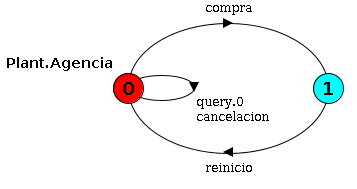
\includegraphics[width=\linewidth]{figures/ejemploServicios/agencia.png}  
		\caption{agencia}
		\label{fig:agencia}
	\end{subfigure}
	\begin{subfigure}[t]{.5\textwidth}
		\centering
		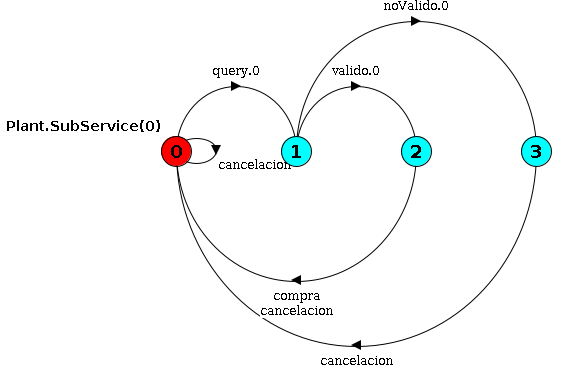
\includegraphics[width=\linewidth]{figures/ejemploServicios/subServicio.png}  
		\caption{un sub servicio}
		\label{fig:subserv}
	\end{subfigure}
	}
	\makebox[\linewidth][c]{%
	\begin{subfigure}[t]{.5\textwidth}
		\centering
		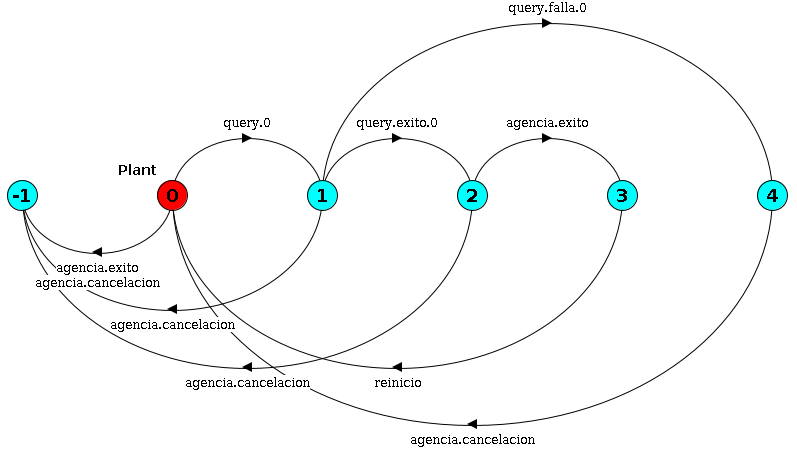
\includegraphics[width=\linewidth]{figures/ejemploServicios/N1Planta.png}  
		\caption{Planta compuesta}
		\label{fig:N1Planta}
	\end{subfigure}
	\begin{subfigure}[t]{.5\textwidth}
	\centering
	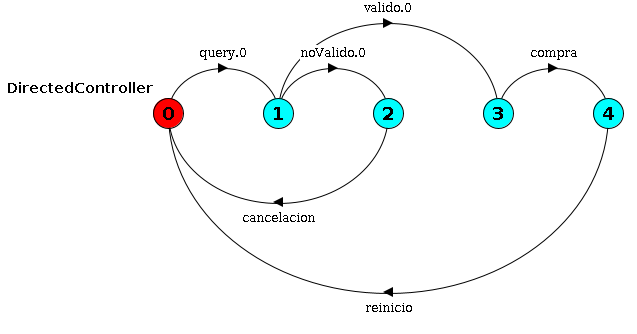
\includegraphics[width=\linewidth]{figures/ejemploServicios/N1Controlador.png}  
	\caption{Controlador resultante}
	\label{fig:controladorN1}
	\end{subfigure}
	}
	\caption{Caso con un solo sub-sevicio}
	\label{fig:N1}
	\end{center}
\end{figure}


\begin{figure}[htb]
	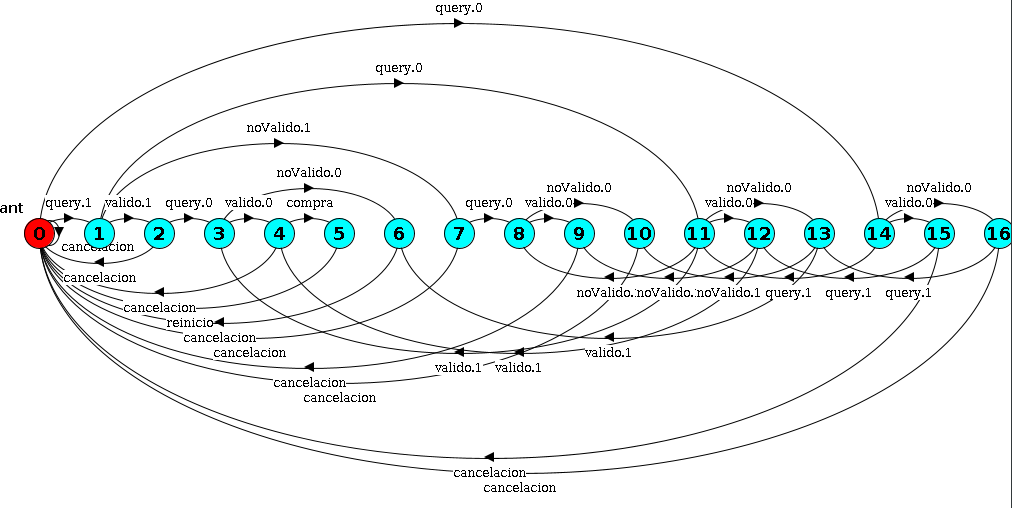
\includegraphics[width=\linewidth]{figures/ejemploServicios/N2Planta.png}  
	\caption{Planta compuesta con 2 sub-servicios}
	\label{fig:N2}
\end{figure}



















\chapter{Antecedentes}\label{chpt:background}
% DEFINICIONES (ANTECEDENTES)
% def pasos y corridas
% controlador
% vemos en particular problemas non-blocking (i.e. loop para ganadores, no-controlables no joden)
% estados ganadores y perdedores (estados desde donde hay una estrategia==controlador ganadora/perdedora)
%-------------------------------------------------------
\begin{frame}{Acciones, pasos y corridas (run)}
    \begin{figure}
        \begin{overprint}
        \onslide<1>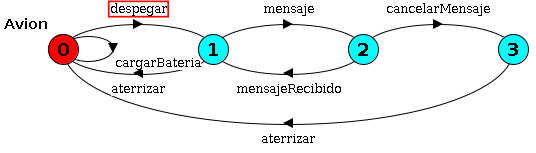
\includegraphics[width=\textwidth]{figures/1accion.png} 
        \onslide<2>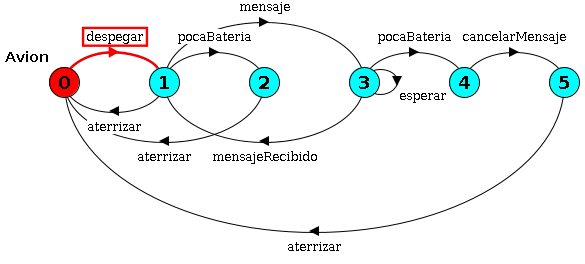
\includegraphics[width=\textwidth]{figures/2paso.png} 
        \onslide<3->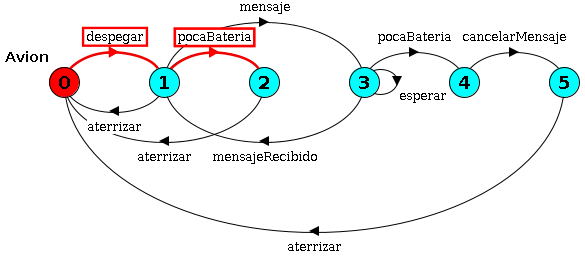
\includegraphics[width=\textwidth]{figures/3run.png} 
        \end{overprint}
    \end{figure}

    \begin{itemize}
     \item Acción es una transición entre los estados.
     \pause
     \item Un paso es $t \step{\l}{T} t'$, toma en cuenta el estado de partida y llegada.
     \pause
     \item Una corrida de una palabra $w = \l_0,\ldots,\l_k$ en $T$, es $t_0 \runw{w}{T} t_{k+1}$, es decir, varios pasos.
    \end{itemize}
    
\end{frame}
%-------------------------------------------------------
\begin{frame}{Problema de control non-blocking}
    \begin{block}{¿Cuál es la entrada de un problema de control?}
        \begin{itemize}
          \item conjunto de autómatas (la composición de ellos es la planta completa que no queremos calcular)
          \item acciones controlables y no controlables
          \item estados marcados u objetivos (se quiere tener la \textit{posibilidad} de visitar infinitas veces \textit{al menos uno})
        \end{itemize}
    \end{block}

    \begin{block}{¿Qué devuelve?}
        Una estrategia ganadora (llamada controlador) o afirmación de que no existe.
    \end{block}

\end{frame}
%-------------------------------------------------------
\begin{frame}{En nuestro ejemplo}
    \begin{description}
     \item[Conjunto de autómatas] Avión, Batería.
     \item[Acciones controlables] despegar, aterrizar, mensaje, cargarBateria, cancelarMensaje.
     \item[Acciones no-controlables] mensajeRecibido, pocaBateria.
     \item[Objetivo] Enviar \textit{mensaje}.
    \end{description}
    
    \textbf{Planta} (composición de todos los autómatas)
    \begin{figure}
     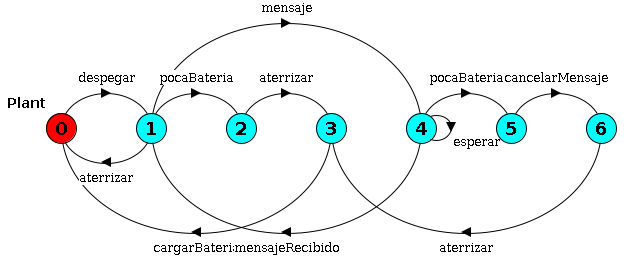
\includegraphics[width=\textwidth]{figures/planta.png}
    \end{figure}
    
\end{frame}
%-------------------------------------------------------
\begin{frame}{Controlador}
    \begin{figure}
     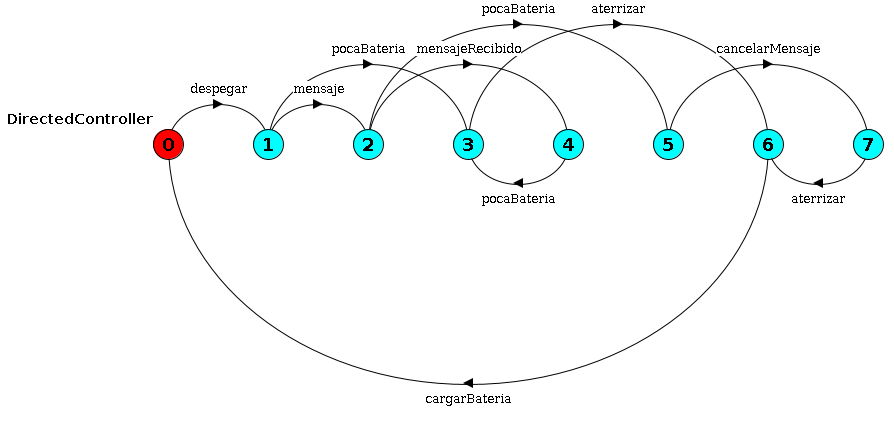
\includegraphics[width=\textwidth]{figures/director.png}
    \end{figure}

    Es una restricción de la planta que cumple las reglas:

    \begin{itemize}
     \item Puede prohibir pasos controlables.
     \item Mantiene todas las acciones no-controlables.
     \item Todas las corridas posibles en la planta restringida pasan por algún estado marcado.
    \end{itemize}
\end{frame}
%-------------------------------------------------------
\begin{frame}{Estados ganadores y perdedores}
	
	\begin{wrapfigure}{r}{0.48\textwidth}
		\vspace{-1cm}
		\hspace{-0.8cm}
		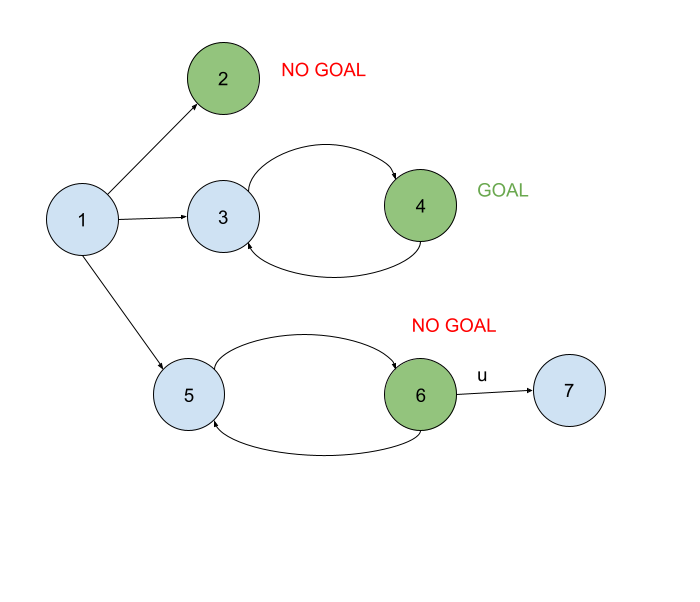
\includegraphics[width=0.6\textwidth]{figures/como-marcar-goals-FACAS.png}
	\end{wrapfigure}
	
    Si existe un controlador comenzando desde un estado, es decir, existe estrategia ganadora a partir del estado, entonces lo consideramos estado ganador. 
    Caso contrario, el estado es perdedor y debemos evitarlo.
    
    \vspace{0.5cm}
    \begin{block}{Observación}
        En particular nos interesa mucho si el estado inicial es ganador/perdedor, ya que eso nos dice si existe o no un controlador \textit{empezando} desde ahí.
    \end{block}

\end{frame}
%-------------------------------------------------------


\chapter{Exploración on-the-fly}\label{chpt:on-the-fly}
El problema de síntesis de controlador ya tiene una solución clásica, por lo que la dificultad del trabajo no consistió en desarrollar un algoritmo que detectara estados ganadores y perdedores de una composición de LTS totalmente explorada. 

El conflicto reside en que al componer distintos DES, la cantidad de estados de la composición es exponencial respecto de los estados en los componentes. Esto es de suma relevancia ya que la solución clásica, que compone toda la planta para luego explorarla, tiene un límite de escalabilidad en el cual la composición de la planta llega al límite de tiempo o memoria, y nunca se llega a la exploración.

Para combatir esto, la exploración on-the-fly, presentada en \cite{tesisDani}, clasifica estados como ganadores o perdedores durante la composición. Se espera que con esto sea posible, en primer lugar, cortar la exploración de una rama de la planta que ya se sabe que es perdedora o ganadora, reduciendo así la memoria y tiempo necesarios. Pero más aún, si el estado inicial fuera marcado como ganador o perdedor antes de la composición completa de la planta, ni siquiera sería necesario completar el proceso de composición.

En el listing \ref{lst:basic_on-the-fly} mostramos la estructura básica de este método. Trabajando sobre la parte de la planta compuesta hasta el momento (estructura explorada, $\structure$), se expande $\structure$ consiguiendo nueva información hasta que sea seguro si el estado inicial es ganador o perdedor en $E$. Al llegar a esta conclusión se retorna el controlador para $\initial$ en $E$ o se notifica que no es controlable.

\begin{definition}
	[Exploración Parcial] \label{def:unexploredTo}
	Sea $E = (S_E,$ $A_E, \D_E, \init{e}, M_E)$. Decimos que $ES$ es una exploración parcial de $E$ ($ES \subseteq E$) si $S_\structure \subseteq 
	S_E$ y $\structure = (S_\structure,A_E, \D_\structure,\init{e},M_E 
	\cap S_\structure)$, donde $ \D_\structure \subseteq (\D_E \cap 
	(S_\structure \times A_E \times S_\structure))$. Escribimos $ES \subset E$ cuando $S_\structure \subset S_E$.
\end{definition}

\begin{lstlisting}[language={pseudocode},label={lst:basic_on-the-fly},caption={Algoritmo on-the-fly básico},float=ht]
Algorithm basicOTF-Exploration($E, A_E^C$):
  $\initial$ = $\<\init{e}^0,\ldots,\init{e}^n\>$
  $\structure = (S_\structure,A_E, \D_\structure,\init{e},M_E 
  \cap S_\structure) \ldot ES \subseteq E$
  until surelyWinsOrLoses($\initial$):
    expandES()
    computeNewWinnersAndLosers($\structure$)
  if $initial \in \Goals$:
    return buildController($\initial$)
  else:
    return "UNREALIZABLE" 
\end{lstlisting}

Puede haber muchas variantes de cada una de estas partes, cómo se expande, cómo se computan nuevos ganadores y perdedores, etc. En particular, nuestro enfoque se muestra en el listing \ref{lst:on-the-fly} y consiste en ir agregando una transición a la vez a la parte conocida de la planta, y en cada paso ver si esta nueva transición permite concluir que un estado es ganador o perdedor. Si algún nuevo estado se clasifica como ganador  o perdedor, se propaga esta información a sus antecesores, posiblemente marcándolos a su vez como ganadores o perdedores, respectivamente.

A medida que exploramos mantenemos dos conjuntos de estados de $\structure$ ($\Goals$ y $\Errors$) para los cuáles ya se tiene una conclusión, es decir, se sabe que son ganadores (o perdedores) en $E$.

Como se demostrará en el capítulo \ref{chpt:dcs}, al expandir $\structure$ con una transición $(e,\l,e')$ a la vez, a menos que $e'$ ya fuera un ganador/perdedor entonces solo puede haber nueva información si existe un loop entre $e$ y $e'$. Es más, si hay un nuevo estado ganador/perdedor, entonces $e$ seguramente es también un nuevo ganador/perdedor, y todos los nuevos estados clasificados son antecesores de $e$. Ésto permite optimizar la detección de nuevos ganadores/perdedores en lugar de ejecutar un algoritmo clásico sobre todo $\structure$.




Para explicar el algoritmo y argumentar su correctitud y completitud introducimos dos nuevos problemas de control para exploraciones parciales. Uno toma una visión optimista de la región no explorada ($\top$) asumiendo que todas las transiciones no exploradas llevan a un estado ganador. El otro toma una visión pesimista ($\bot$) asumiendo que las transiciones no exploradas llevan a estados perdedores.

\begin{definition}
	[Problemas de Control $\top$ y $\bot$] \label{def:unexploredTo}
	
	Sean $\E = (E, A_E^C)$, $E = (S_E,A_E,\D_E,\init{e},M_E)$ y $\structure = 
	(S_\structure,A_E, \D_\structure,\init{e},M_E \cap S_\structure)$, y $\structure 
	\subseteq E$.
	\\
	Definimos $\E_\top$ como $(\unexploredToTop{\structure}, A_E^C)$ donde 
	$\unexploredToTop{\structure} = (S_\structure \cup \, \{\top\},A_E,\D_\top, 
	\init{e}, 
	(M_E \cap S_\structure)\, \cup \, \{\top\})$ y $\, \D_\top \, = \, \D_\structure 
	\, 
	\cup\, \{(s,\l, \top) 
	\;$ $ | \; \exists s' \ldot (s, \l, s') \in (\D_E \setminus \D_\structure)\} \cup \{(\top, \l, \top) \, | \, \l \in A_E\}$ \\
	Definimos $\E_\bot$ como $(\unexploredToBottom{\structure}, A_E^C)$ donde 
	$\unexploredToBottom{\structure} = (S_\structure \, \cup \, 
	\{\bot\},A_E,\D_\bot, 
	\init{e}, M_E \cap S_\structure)$ y $\D_\bot = \D_\structure \, \cup \, \{(s,\l, 
	\bot) \, | \, $ $ \exists s' \ldot (s, \l, s') \in (\D_E \setminus \D_\structure)\}$ 
\end{definition}

Usamos estos problemas de control para decidir tempranamente si un estado $s$ es ganador o perdedor en $E$ basado en lo que exploramos previamente en $\structure$. Si $s$ es ganador en $\unexploredToBottom{\structure}$ esto significa que sin importar a dónde lleven las transiciones no exploradas, $s$ también va a ser ganador en $E$. Similarmente, $s$ es perdedor en $E$ si es perdedor en $\unexploredToTop{\structure}$.
El Lema~\ref{lem:WESandLesMonotonicity} refuerza este razonamiento.


\begin{lemma}\textbf{\emph{(Monotonicidad de $\WES$ y $\LES$)}}
	\label{lem:WESandLesMonotonicity}
	Sean $\structure$ y $\structure'$ dos exploraciones parciales de $E$ tal que $\structure 
	\subset \structure'$ entonces $\WES \subseteq \WESS$ y $\LES \subseteq 
	\LESS$.
\end{lemma}

El algoritmo agrega iterativamente una transición de $E$ a $\structure$ a la vez y asegura que al final de cada iteración, los estados en $\structure$ están correcta y completamente clasificados en ganadores y perdedores si hay suficiente información de $E$ en $\structure$. Los conjuntos de estados $Errors$, 
$Goals$ y $\NONE$ se usan para este propósito.



En el peor caso, si no se pudo concluir nada antes de componer la planta en su totalidad, se perdió tiempo en los puntos fijos, intentando clasificar estados, y se realiza una última vez el algoritmo clásico con la planta totalmente explorada. Esto garantiza la completitud del algoritmo, como se detalla en mayor profundidad en el capítulo~\ref{chpt:dcs}.

\begin{lstlisting}[language={pseudocode},label={lst:on-the-fly},caption={Nuestro enfoque on-the-fly},float=ht]
Algorithm genericOTF-Exploration($E, A_E^C$):
   $\initial$ = $\<\init{e}^0,\ldots,\init{e}^n\>$
   $\Goals = \Errors = \emptyset$
   $\structure = initial$ //la parte conocida de la planta
   while $initial \notin \Goals \cup \Errors$:
     $(e,\l,e') = $nextTransition($\structure, heuristica$)
     expandES($\structure,(e,\l,e')$)
     if $e' \in \Errors$:
       propagateError($e'$)
     else if $e' \in \Goals$:
       propagateGoal($e'$)
     else if isLoop($e,e'$):
       if newWinningLoop($e,e'$):
         propagateGoal($e'$)
       else if newLosingLoop($e,e'$):
         propagateError($e'$)
         
   if $initial \in \Goals$:
     return buildController($\Goals$)
   else:
     return "UNREALIZABLE"  
\end{lstlisting}

Para explorar en el orden más conveniente, y componer una menor parte de la planta, se utiliza una heurística de exploración Best First Search \cite{tesisDani}. La misma busca ganar controlablemente o perder no controlablemente, para garantizar con la menor exploración posible que el estado actual es ganador o perdedor.

Una heurística no presenta garantía de explorar en la dirección correcta, más bien da una recomendación. Son ampliamante utilizadas al optimizar, pero es importante que la correctitud de los algoritmos no dependan de estas recomendaciones, ya que por su misma naturaleza no tienen garantías fuertes.

\section{Agnosticismo a la heurística}

Una distinción clave del algoritmo \textit{on-the-fly} es que está dividido en dos partes. Por un lado se tiene el algoritmo de exploración responsable de que al final se llegue al resultado correcto, por el otro tenemos una heurística que le brinda la próxima transición a explorar. Ese algoritmo de exploración no puede depender de la heurística, ya que la misma no garantiza siempre elegir el mejor camino posible, sino solo la mejor aproximación que encuentre. Uno de los focos de nuestro trabajo fue en esa corrección independiente del orden de exploración de las transiciones.

El proyecto \texttt{MTSA} inicialmente contaba con dos heurísticas \texttt{Best First Search} para exploración, \textit{Monotonic Abstraction} y \textit{Ready Abstraction}. 

El inconveniente con la versión anterior del algoritmo de exploración es que había sido desarrollado en conjunto con las heurísticas. Si bien esto ayudaba a la eficiencia del mismo, generaba una dependencia del orden de observación de las transiciones, dando resultados erróneos al cambiar las recomendaciones. El nuevo enfoque no depende de la forma de explorar, por ende, da una mayor libertad de investigar a futuro nuevos criterios de evaluación para mejorar la eficiencia de la técnica sin comprometer corrección ni completitud. Esto fue útil durante el desarrollo del trabajo, ya que facilitó la inclusión de nuestras nuevas heurísticas (\texttt{Dummy} y \texttt{Breadth First Search}, ver sección \ref{chpt:heurist-nuevas}) para la experimentación.


\section{Ejemplo de ejecución}

Para ilustrar el funcionamiento y ventajas de la exploración on-the-fly, mostramos una ejecución posible sobre una planta ejemplo. Supongamos que dados ciertos autómatas calculamos su composición y llegamos a la planta de la figura \ref{fig:ej:plantaCompleta}. Las transiciones se van a explorar en orden de menor a mayor, en el diagrama las (u)/(c) son no controlables/controlables respectivamente y el estado marcado tiene doble círculo. No especificamos la controlabilidad de todas las transiciones de manera de hacer más legible el gráfico y además porque, mirando las definidas, no nos modifica la conclusión el hecho de que sean o no controlables. %TODO ok esto no? es confuso? lo sacamos?  

\begin{figure}
 \centering
 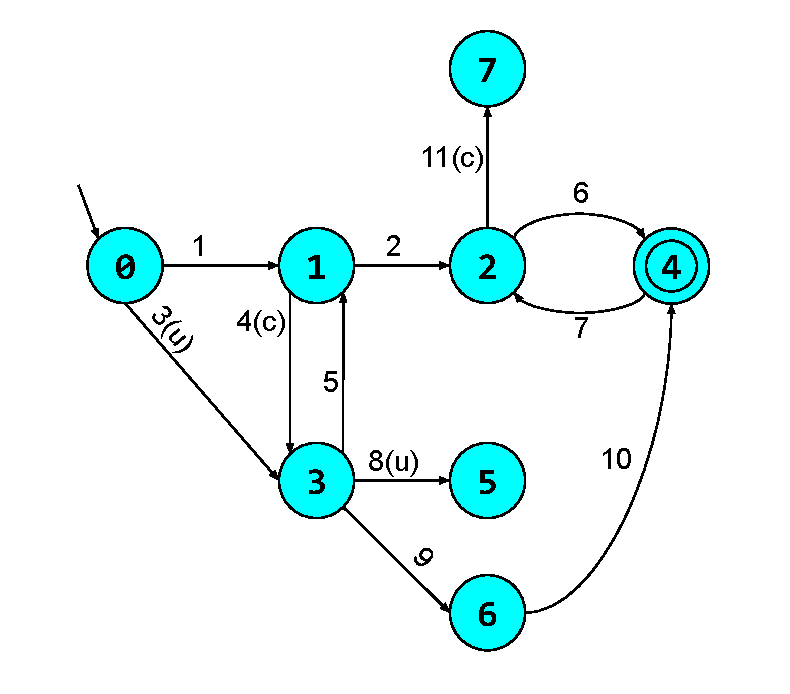
\includegraphics[scale=0.6]{figures/ejemplo_on-the-fly/0.pdf}
 \caption{Planta compuesta completa}
 \label{fig:ej:plantaCompleta}
\end{figure}

Al iniciar el algoritmo no vemos la planta completa sino sólo el primer estado \cyan{0}, desde el mismo expandimos la primer transición, en este caso \textit{1}. Como llega a un estado sin explorar \cyan{1}, y que no es deadlock, no hay información para conseguir. Entonces mientras lleguemos a ``algo nuevo'' no tenemos nada para hacer más que seguir explorando.
Incluso si llegamos a un estado explorado (no deadlock) no va a haber nueva información si no tenemos un loop. Veremos más en detalle y con demostración por qué esto es así en el capítulo \ref{chpt:dcs}; pero la intuición es que no va a haber nuevos ganadores puesto que un ganador necesita llegar a un marcado infinitas veces, por ende necesita como mínimo que haya un loop. Entonces hasta ahora llevamos explorado lo mostrado en la figura \ref{fig:ej:exploracion1}.

\begin{figure}[h]
 \centering
 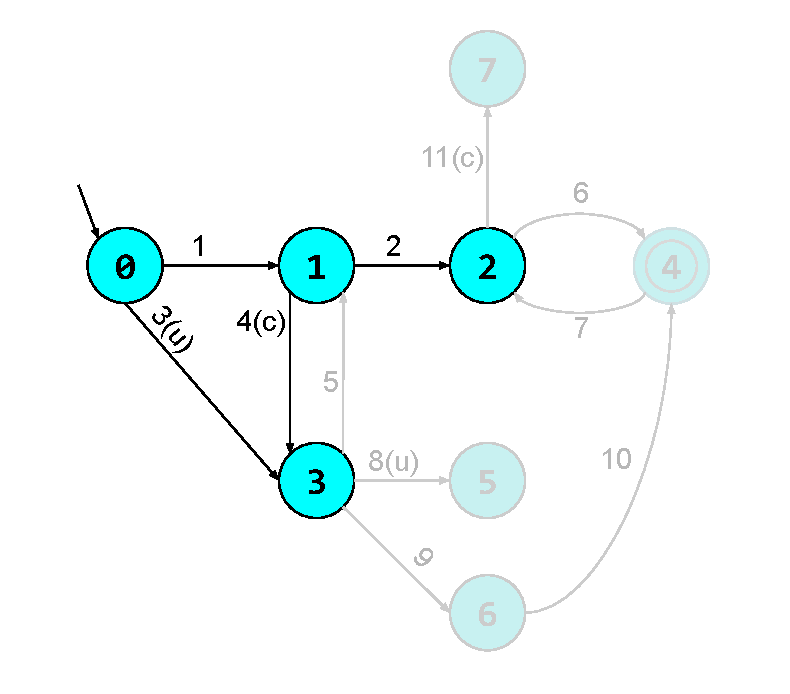
\includegraphics[scale=0.6]{figures/ejemplo_on-the-fly/1.pdf}
 \caption{Primeros pasos de exploración}
 \label{fig:ej:exploracion1}
\end{figure}

Si seguimos explorando por la transición \textit{5} cerramos un loop [\cyan{1}, \cyan{3}], pero \cyan{3} puede ser forzado a algo no explorado usando la transición no controlable \textit{8}, entonces todavía no podemos sacar conclusión alguna. Exploramos hasta figura \ref{fig:ej:exploracion2}.

\begin{figure}
 \centering
 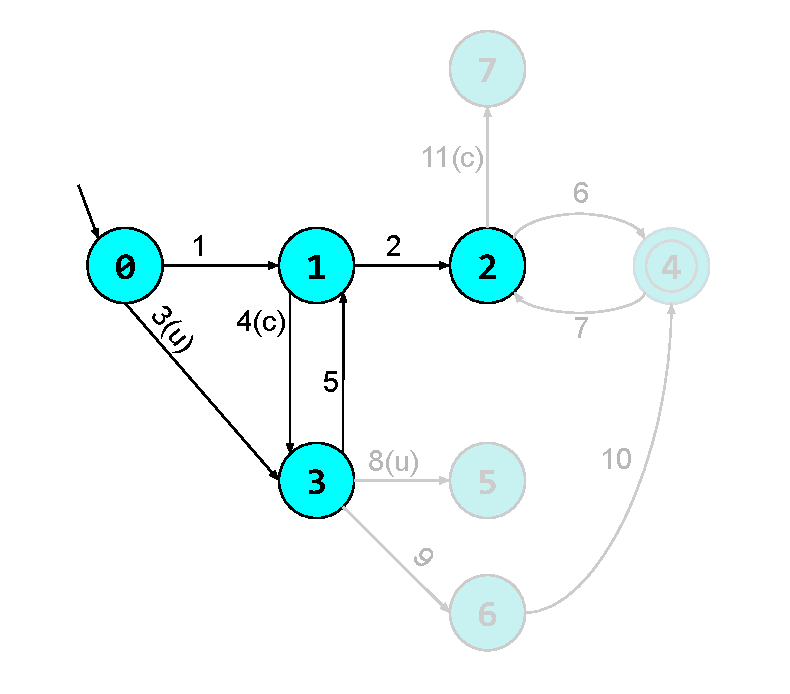
\includegraphics[scale=0.6]{figures/ejemplo_on-the-fly/2.pdf}
 \caption{Hay loop sin conclusiones nuevas}
 \label{fig:ej:exploracion2}
\end{figure}

Continuamos y llegamos a un estado marcado \cyan{4}, si fuese sólo alcanzar un marcado podríamos decir que es ganador pero necesitamos siempre poder llegar a uno (incluso desde sí mismo), por ende ahora sigue sin ser nada. Luego vemos \textit{7}, cerrando loop [\cyan{2}, \cyan{4}]. Éste loop tiene un estado marcado y \cyan{2} no puede ser forzado a otra cosa, ya que el resto de sus transiciones son controlables; por ende obtenemos nuestros primeros ganadores (\cyan{2} y \cyan{4}). A continuación debemos propagar esta nueva información llegando a marcar \cyan{1} como ganador, porque puede controlablemente llegar al loop [\cyan{2}, \cyan{4}]. Lamentablemente todavía no hay conclusión sobre el estado inicial debido a que puede ser forzado a algo sin explorar. Ver figura \ref{fig:ej:exploracion3}.

\begin{figure}[h]
 \centering
 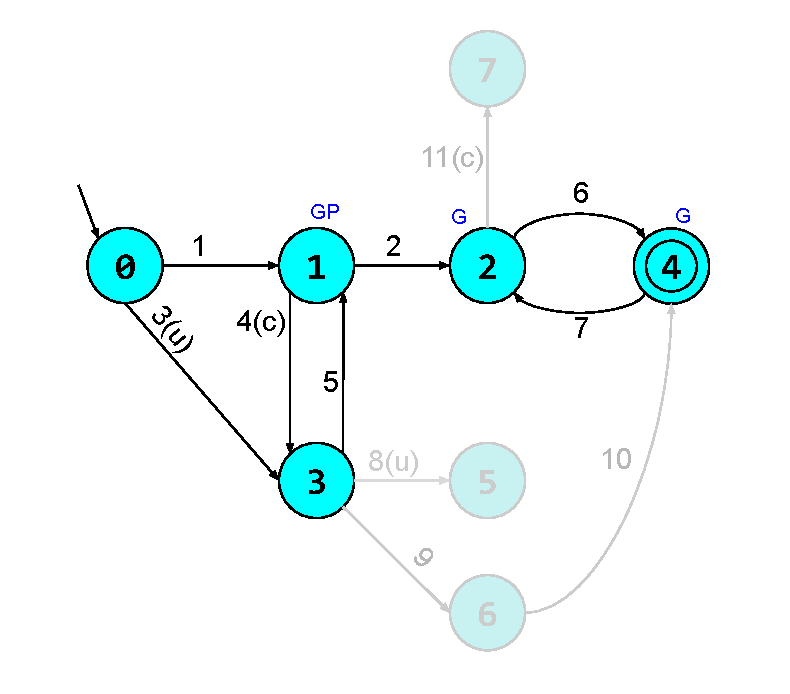
\includegraphics[scale=0.6]{figures/ejemplo_on-the-fly/3.pdf}
 \caption{Se encuentra Goal [2, 4] y propaga (1)}
 \label{fig:ej:exploracion3}
\end{figure}

Proseguimos con \textit{8} y llegamos a explorar el estado \cyan{5}, que es un deadlock por ende es error directamente. Propagando esta información marcamos los estados \cyan{3} y \cyan{0} como errores, llegando así a una conclusión sobre el inicial. Entonces ya no nos es necesario seguir explorando y se retorna que \textit{no existe controlador para la planta}. El estado de exploración final de la planta se ve en la figura \ref{fig:ej:exploracion4}.

\begin{figure}
 \centering
 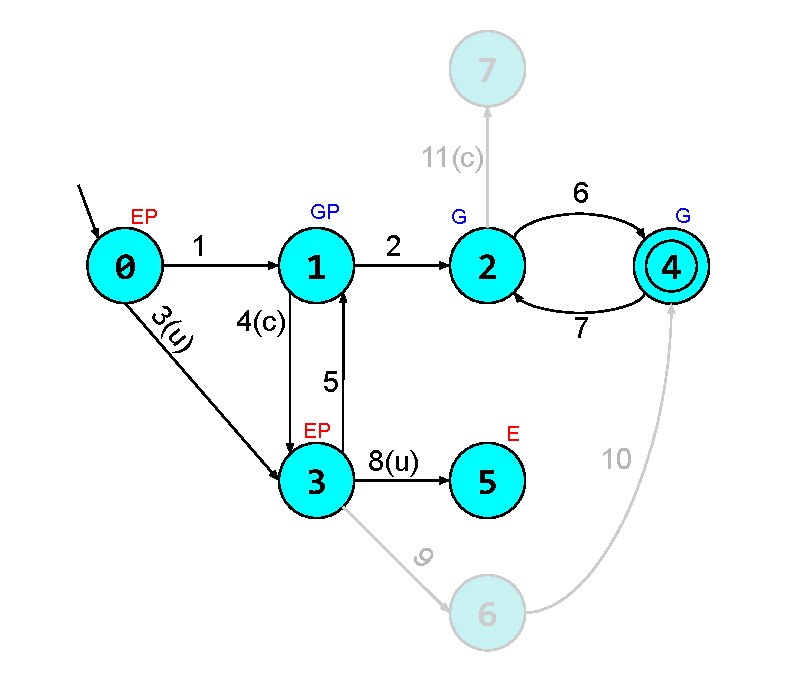
\includegraphics[scale=0.6]{figures/ejemplo_on-the-fly/4.pdf}
 \caption{Se encuentra Error (5) y propaga hasta inicial (3, 0), dejando de explorar}
 \label{fig:ej:exploracion4}
\end{figure}

Notar que no vemos las demás transiciones de \cyan{2} ni \cyan{3} ya que, en el caso de \cyan{2} gana por alguna y el resto son controlables, y en el caso de \cyan{3} pierde por una no controlable. Es decir, \cyan{2} puede controlablemente ganar y \cyan{3} es forzado a perder sin importar la forma del resto.

Si la transición \textit{8} fuese controlable podríamos evitar el error y seguiríamos explorando, encontrando el estado \cyan{6}, su conexión al loop ganador y propagando ganador hasta el estado inicial. Notar que ésta sería una planta \textit{diferente}, controlable a diferencia de la propuesta en el ejemplo.












%\section{Invariante}\label{sct:invariante}

%Intentando resolver el problema del marcado explícito de errores, buscamos una separación fuerte entre los estados $error \in L_E$ y los estados para los cuales no tenemos suficiente información para clasificar en este momento $\NONE$. Para esto, los lemas detallados en la sección de demostración del algoritmo aseguran que un estado marcado como ganador o perdedor lo es en la planta compuesta totalmente explorada, y nunca puede cambiar su estado.

%Como se verá en la propiedad~\ref{def:invariant} del siguiente capítulo, un estado $s$ solo puede seguir sin clasificar (siendo $\NONE$) si, con los explorados hasta el momento, y siendo totalmente optimistas sobre las transiciones desconocidas no podemos asegurar que $s$ está condenado a ser perdedor (y tampoco podemos concluir que es ganador siendo pesimistas).

%Al momento de haber explorado todos los descendientes de $s$, incluso si no se exploró toda la planta total, es claro que no importa si se es optimista ($\top$) o pesimista ($\bot$) para saber si $s$ es un estado ganador o perdedor, por lo que nos forzamos por nuestro invariante a clasificarlo. Con esto evitamos las ramas totalmente exploradas pero sin clasificar que traían complicaciones en la figura~\ref{fig:falenciasErrores} y solo permitimos que un estado sea $\NONE$ si tiene un camino a una transición no explorada.\\





\chapter{Sintesis de Controladores Dirigida}\label{chpt:dcs}
En esta sección presentamos el nuevo algoritmo \DCS, que realiza una exploración sobre la marcha del espacio de estados. Por medio de dicha exploración el algoritmo encuentra una solución al problema composicional de "supervisory control". También discutimos la correctitud y completitud del nuevo algoritmo \DCS. \\

\section{Problemas encontrados}
%En problema con solución actual plantearía entre otras cosas que el best first search tiene que ser correcto para cualquier heuristica y que eso no se cumpía. Plantearía el suite de regresión que armaron y com tuvieron que harnesear el tema de la heuristica para mostrar algunos bugs

ADEMAS EL PROPAGATE NO PODIA SER LOCAL, EXPLICAR.

El anterior algoritmo de exploración tenía falencias en cuanto a agregar estados al conjunto $\Errors$. Esto se debía a que no sacaba conclusión alguna al haber explorado todo un subgrafo, por ende al propagar información desde otra rama se podría llegar a un resultado erroneo. Para comprender mejor observar la figura (INGRESE FIGURA) donde desde el estado e tenemos dos sub-ramas a explorar. Si se mira primero la de abajo y no lo marcamos como error entonces al mirar la de arriba diremos que es goal y propagaremos dicha información, equivocadamente, más allá de e.

Cabe aclarar que sólo podemos concluir que un loop es error cuando este ha sido explorado en su completitud. Esto es así debido a la naturaleza optimista de los problemas non-blocking.

Fue a causa de esta necesidad de marcar errores que decidimos diseñar un nuevo algoritmo con un invariante que consideramos clave para síntesis on-the-fly: Si con la información de lo explorado hasta el momento es posible concluir que un estado es ganador o perdedor en la planta totalmente explorada, debemos marcar ese estado antes de seguir explorando.

EXPLICAR QUE NUESTRO ALGORITMO ES AGNÓSTICO A LA HEURÍSICA (COMO DEBERÍA)

%Subiría de nivel el “Nuevo algoritmo”. Trataría de explicar tempranamente la idea de construcción de núcleos de posibles zonas perdedoras o ganadoras optimistas y pesimistas y la propagación. Incluso con la formalización primero.

\section{Propuesta de nuevo algoritmo}

\lstset{escapeinside={(*@}{@*)}}
\lstset{numbers=left, numberstyle=\tiny, stepnumber=1, numbersep=5pt}
\begin{lstlisting}[language={pseudocode},label={lst:dcs},caption={Algoritmo de exploración dirigida on-the-fly.},float=ht, frame=single]
 function DCS($\E {=} (E, A_E^C)$,$\:\heuristic$):
   $\initial$ = $\<\init{e}^0,\ldots,\init{e}^n\>$
   $\structure = \trimlst{(\{ \initial \}, A_E, \emptyset, \initial, M_E \cap \{\initial\})}$
   $\Goals = \Errors = \Witness = \emptyset$
   $\NONE = \{\initial\}$
   if (isDeadlock($\initial$)):(*@\label{line:initialDead}@*)
   $\Errors = \{\initial\}$
   $\NONE = \emptyset$
   while $\initial \not\in \Errors \cup \Goals$:
     $(e,\l,e')$ = expandNext($\heuristic$) (*@\label{line:expand}@*)
     $S_{\structure'} = S_\structure\cup  \{ e' \}$
     $\structure' = \trimlst{(S_{\structure'} , A_E, \D_\structure \cup \{ e \step{\l}{} e' 
     \}, \initial, M_E \cap S_{\structure'} )}$
     if $e' \in \Errors $: (*@\label{line:isLosing}@*)
       propagateError($\{e'\}$)
     else if $e' \in \Goals$: (*@\label{line:isWinning}@*)
       propagateGoal($\{e'\}$)
     else if canReach($e, e', \structure$): (*@\label{line:isLoop}@*)
       $\SCC$ = getMaxLoop($e$,$e'$) (*@\label{line:getMaxLoop}@*)
       if canBeWinningLoop($\SCC$): (*@\label{line:CanBeWinning}@*)
         C = findNewGoalsIn($\SCC$) (*@\label{line:lookingForWinner}@*)
         $\Witness = \Witness \cup (C \cap M_{\structure'})$
         $\Goals = \Goals \cup C$
         $\NONE = \NONE \setminus C$
         propagateGoal(C)   (*@\label{line:propagateGoal2}@*)
       else:    (*@\label{line:CanBeLosing}@*)
         P = findNewErrorsIn($\SCC$)
         $\Errors = \Errors \cup P$
         $\NONE = \NONE \setminus P$
         propagateError(P) (*@\label{line:propagateError2}@*)
     $\structure = \structure'$
 
   if $\initial \in \Goals$:
     $r = rankStates(\structure)$ (*@\label{line:controller-start}@*)
     $return \, \lambda w \ldot \{ \, \l \mid \trimlst{\initial \runw{w}{\structure} e 
     \step{\l}{\structure} e'} \wedge e' \in \Goals\,$
     $\wedge (l \in A^C_E \then \l = bestControllable(s,r,\structure) 
     )\}$(*@\label{line:controller-end}@*)
   else:
     return UNREALIZABLE
\end{lstlisting}  
%invariante del ciclo:  Inv($states(\structure), \structure)$

\lstset{numbers=none, numberstyle=\tiny, stepnumber=1, numbersep=5pt}
\begin{lstlisting}[language={pseudocode},label={lst:dcs.propagate},caption={Algoritmos de propagación.},float=ht, frame=single]
 function propagateGoal($newGoals$):
   $C' = \emptyset$; $C$ = ancestorsNone($newGoals$)
   while $C'\neq C$:
     $C' = C$
     $C=C \setminus \{ s \in C \mid$ 
       forcedTo($s, S_{\unexploredToBottom{\structure'}}\setminus (C \cup \Goals),\unexploredToBottom{\structure'}$) $\vee$
       cannotReachGoalIn($s, C$)$\}$
   $\Goals = \Goals \cup C$
   $\NONE = \NONE \setminus C$

 procedure propagateError($newErrors$):
   $P$ = ancestorsNone($newErrors$)
   $C$ = $P$; $C' = \emptyset$
   while $C' \neq C$:
     $C' = C$
     $C=C \setminus \{ s \in C \mid$ 
     	forcedTo($s,\Errors,\unexploredToTop{\structure'}$) $\vee$
     	cannotReachGoalIn($s, C$)$\}$
   $P = P \setminus C$
   $\Errors = \Errors\ \cup P$
   $\NONE = \NONE \setminus P$
\end{lstlisting}


\begin{lstlisting}[language={pseudocode},label={lst:dcs.gather},caption={Confirmación de clasificaciones},float=ht, frame=single]
 function findNewGoalsIn($\SCC$):
   $C = \SCC$; $C' = \emptyset$
   while $C' \neq  C:$
     $C' = C$; $C'' = \emptyset$
     while $C'' \neq C:$
       $C'' = C$
       $C=C \setminus \{ s \in C \mid$ 
               forcedTo($s, S_{\unexploredToBottom{\structure'}}\setminus (C \cup \Goals),\unexploredToBottom{\structure'}$) $\vee$
               cannotBeReached($s,C$) $\}$
     $C = C \setminus \{ s \in C \mid $cannotReachGoalOrMarkedIn($s, C$)$\}$
   return C
  
 function findNewErrorsIn($\SCC$):
   if ($\exists s \in \SCC \ldot \trimlst{s \step{\l'}{\unexploredToTop{\structure'}}  s'} 
   \wedge (s' \notin \SCC \wedge s' \notin \Errors)$):
     return $\emptyset$
   else: 
     return $\SCC$
\end{lstlisting}



%VErsion anterior
%   let $(e,\l,e')\in (\D_{E}\setminus\D_{\structure})$ such that $e\in S_\structure\ 
%   \wedge$
%     ($\forall (s,\l',s')\in (\D_{E}\setminus\D_{\structure})\, s\in S_\structure \ldot$ 
%        $\heuristic$($e, \l, e'$) $>=$ $\heuristic$($s, \l', s'$))

% AUX FUNCTIONS
\begin{lstlisting}[language={pseudocode},label={lst:dcs.aux},caption={Métodos auxiliares},float=ht, frame=single]
 procedure expandNext($\heuristic$):
   let $\trimlst{(e,\l,e') \ldot e\in S_\structure \wedge e\step{\l}{E} e' \wedge   
       \neg e\step{\l}{\structure} e' \wedge e \in \NONE \wedge}$ 
       $\trimlst{\forall (s,\l',s') \ldot  s\in S_\structure \wedge s\step{\l}{E} s' \wedge \neg s\step{\l}{\structure} s' \wedge s \in \NONE}$ 
         $\implies \trimlst{\heuristic(e, \l, e') >=\heuristic(s, \l',   s'))}$
   if isDeadlock($e'$):
     $\Errors$ = $\Errors \cup \{e'\}$
   if $e'\notin \Errors \cup \Goals$:
     $\NONE = \NONE \cup \{e'\}$
   return $(e,\l,e')$
 
 function ancestorsNone(targets):
   return $\{ \, e \in \structure' \mid \exists e' \in targets \ldot \exists w \ldot \trimlst{e \runw{w}{\structure'} e'} \wedge$
          $ \nexists s \in w(e) \ldot s \neq e' \wedge \in \Goals \cup \Errors \}$
   
 function canBeWinningLoop(loop):
   return $(\marked{loop}{\structure'}) \vee$ 
          $(\exists s \in loop \ldot $canReachInOneStep($s, \structure, \Goals$)$)$
   
 function getMaxLoop($e$,$e'$):
   return $\{s \mid \exists w, w' \ldot \trimlst{e \runw{w}{\structure'} s} \wedge \trimlst{s \runw{w'}{\structure'} e'} \wedge$ 
          $\nexists s' \ldot (s' \in w(e) \vee s' \in w'(s)) \wedge s' \neq e' \wedge s' \in \Goals \cup \Errors \}$

 function forcedTo($s,Dest,Z$):
   return $(\exists \l_u \in A_Z^U \ldot \exists e \in Dest \ldot \trimlst{s \step{\l_u}{Z} e})\ \vee$
          $(\forall \l \in A_Z \  (\trimlst{s \step{\l}{Z} e} \Rightarrow e \in Dest))$    
    
 function cannotBeReached($s, C$):
    return $\nexists s' \in C , \exists \l \ldot s' \step{\l}{\structure'} s$
   
 function cannotReachGoalOrMarkedIn($s, C$)
    return $\trimlst{\nexists w \ldot s \runw{w}{C} s' \wedge s'\in C\ \wedge}$ 
           $($canReachInOneStep$(s', \structure, \Goals)$
           $\vee\ s'\in\M_{\structure'})$
           
 function cannotReachGoalIn($s, C$)
    return $\trimlst{\nexists w \ldot s \runw{w}{C} s' \wedge s'\in C\ \wedge}$ 
           canReachInOneStep$(s', \structure, \Goals)$
           
 function canReach($s', s$)
    return $\exists w \ldot s' \runw{w}{\structure'} s$

 function canReachInOneStep($s, Targets$)
    return $\exists l \ldot s \step{\l}{\structure'} s' \wedge s' \in Targets$

 function isDeadlock($s$)
    return $\nexists l \ldot s \step{\l}{E} s'$
\end{lstlisting}

\begin{lstlisting}[language={pseudocode},label={lst:dcs.aux},caption={Métodos de ranking},float=ht, frame=single]
 function rankStates($\structure$)
    $r = 0$; $W' = \Witness$; $W = \emptyset$
    while $W' \neq  W:$
      $\forall w \in W', $rank$(w) = r$
      $W = W \cup W'$
      $W'= \{ s \in (\Goals \setminus W) \mid \exists s' \in W \ldot s \step{}{\structure} s'\}$
      $r = r + 1$
    return rank

 function bestControllable($e, r, \structure$)
    return $\l \in A^C_E \ldot e \step{\l}{\structure} e' \wedge \nexists \l' \in A^C_E \ldot $
			$e \step{\l'}{\structure} e'', r(e'') \leq r(e')$

\end{lstlisting}


%
% function isDeadlock($e$):
%   return $\neg\exists \l \! \ldot \trimlst{e \step{\l}{E} e'}$
%
% function canReach($e, e', Z$):
%   return $\exists w \ldot \trimlst{e' \runw{w}{Z} e}$
%   
% function canReachInOneStep($s, Z, \S$):
%   return $\trimlst{\exists l \ldot s \step{\l}{Z} s' \wedge s' \in \S}$

\FloatBarrier

\section{Demostración de corectitud y completitud}
\begin{notation}
Decimos que un estado $s$ es ganador["winning"] (resp. perdedor["losing"]) en el problema $\E = 
(E, A_E^C)$ siendo $s$ el estado inicial de $E$ si hay una (resp. no hay una) solución para $\E$. Nos referimos a los estados ganadores y perdedores de $E$ cuando $A_E^C$ es inferible del contexto, también usamos $W_E$ y $L_E$ para denotar el conjunto de estados ganadores y perdedores de $\E$.
\end{notation}

El algoritmo (ver Listing~\ref{lst:dcs}) explora incrementalmente el espacio de estados de $E$ utilizando una estructura de exploración parcial ($ES$), añadiéndole una transición por vez.


\begin{definition}
[Exploración Parcial] \label{def:unexploredTo}
Sea $E = (S_E,$ $A_E, \D_E, \init{e}, M_E)$. Decimos que $ES$ es una exploración parcial de $E$ ($ES \subseteq E$) si $S_\structure \subseteq 
S_E$ y $\structure = (S_\structure,A_E, \D_\structure,\init{e},M_E 
\cap S_\structure)$, donde $ \D_\structure \subseteq (\D_E \cap 
(S_\structure \times A_E \times S_\structure))$. Escribimos $ES \subset E$ cuando $S_\structure \subset S_E$.
\end{definition}

Para explicar el algoritmo y argumentar su correctitud y completitud introducimos dos nuevos problemas de control para exploraciones parciales. Uno toma una visión optimista de la región no explorada ($\top$) asumiendo que todas las transiciones no exploradas llevan a un estado ganador. El otro toma una visión pesimista ($\bot$) asumiendo que las transiciones no exploradas llevan a estados perdedores.

\begin{definition}
[Problemas de Control $\top$ y $\bot$] \label{def:unexploredTo}

Sean $\E = (E, A_E^C)$, $E = (S_E,A_E,\D_E,\init{e},M_E)$ y $\structure = 
(S_\structure,A_E, \D_\structure,\init{e},M_E \cap S_\structure)$, y $\structure 
\subseteq E$.
\\
Definimos $\E_\top$ como $(\unexploredToTop{\structure}, A_E^C)$ donde 
$\unexploredToTop{\structure} = (S_\structure \cup \, \{\top\},A_E,\D_\top, 
\init{e}, 
(M_E \cap S_\structure)\, \cup \, \{\top\})$ y $\, \D_\top \, = \, \D_\structure 
\, 
\cup\, \{(s,\l, \top) 
\;$ $ | \; \exists s' \ldot (s, \l, s') \in (\D_E \setminus \D_\structure)\} \cup \{(\top, \l, \top) \, | \, \l \in A_E\}$ \\
Definimos $\E_\bot$ como $(\unexploredToBottom{\structure}, A_E^C)$ donde 
$\unexploredToBottom{\structure} = (S_\structure \, \cup \, 
\{\bot\},A_E,\D_\bot, 
\init{e}, M_E \cap S_\structure)$ y $\D_\bot = \D_\structure \, \cup \, \{(s,\l, 
\bot) \, | \, $ $ \exists s' \ldot (s, \l, s') \in (\D_E \setminus \D_\structure)\}$ 
\end{definition}

Usamos estos problemas de control para decidir tempranamente si un estado $s$ es ganador o perdedor en $E$ basado en lo que exploramos previamente en $\structure$. Si $s$ es ganador en $\unexploredToBottom{\structure}$ esto significa que sin importar a dónde lleven las transiciones no exploradas, $s$ también va a ser ganador en $E$. Similarmente, $s$ es perdedor en $E$ si es perdedor en $\unexploredToTop{\structure}$.
Lemma~\ref{lem:WESandLesMonotonicity} refuerza este razonamiento.


\begin{lemma}\textbf{\emph{(Monotonicidad de $\WES$ y $\LES$)}}
\label{lem:WESandLesMonotonicity}
Sean $\structure$ y $\structure'$ dos exploraciones parciales de $E$ tal que $\structure 
\subset \structure'$ entonces $\WES \subseteq \WESS$ y $\LES \subseteq 
\LESS$.
\end{lemma}

El algoritmo agrega iterativamente una transición de $E$ a $\structure$ a la vez y asegura que al final de cada iteración, los estados en $\structure$ están correcta y completamente clasificados en ganadores y perdedores si hay suficiente información de $E$ en $\structure$. Los conjuntos de estados $Errors$, 
$Goals$ y $\NONE$ se usan para este propósito.

\begin{property}[Invariante]
\label{def:invariant}
El loop principal del Algorithm~\ref{lst:dcs} tiene el siguiente invariante: 
$\structure \subseteq E \ \wedge $ $\forall s \in \structure \ldot (s\in\Goals 
\Leftrightarrow 
s \in 
\WES)$ $\wedge$  $(s\in\Errors 
\Leftrightarrow s \in \LES)$ $\wedge$  
$s\in\Errors\uplus\Goals\uplus\NONE$

% \begin{tabbing}
% ajfdlkadl\= \kill
% \> \= 
% \>$s\in\Goals \Leftrightarrow s \in \WES \wedge$ \\
% \> $s\in\Errors \Leftrightarrow s \in \LES \wedge$ \\
% \> $s\in\Errors\uplus\Goals\uplus\NONE$
% \end{tabbing}
\end{property}

La explicación del Algorithm~\ref{lst:dcs} que detallamos a continuación sirve también como un esquema de demostración para Property~\ref{def:invariant}.   

Para empezar, notar que la función \texttt{expandNext} 
(line~\ref{line:expand}) retorna una nueva transición $e \step{\l}{E} e'$ 
garantizando que $e$ ya se encontraba en $\structure$ y $e \in \NONE$. 
Esto significa que en cada iteración, hay algo de información nueva disponible para un estado que actualmente no está clasificado en ganador ni perdedor.

Si el estado $e'$ ya es clasificado como ganador en
$\unexploredToBottom{\structure}$ (line~\ref{line:isWinning}) o
perdedor en $\unexploredToTop{\structure}$ (line~\ref{line:isLosing}) 
entonces esta información necesita ser propagada a los estados en $\NONE$ para ver si pueden convertirse en ganadores en 
$\unexploredToBottom{\structure'}$ o perdedores en
$\unexploredToTop{\structure'}$. Tanto \texttt{propagateGoal} como
\texttt{propagateError} realizan un punto fijo estándar~\cite{Ramadge:1989:CDES} sobre
$\unexploredToBottom{\structure}$ y
$\unexploredToTop{\structure}$ pero solo sobre predecesores de $e'$ que están en $\NONE$. 
Lemma~\ref{lem:newWinnersLosersAreNonePredecessors} asegura la completitud de esta propagación restringida.

%Hack de titulo de lemma porque si no, no corta linea.
\begin{lemma}\textbf{\emph{(Ganadores/Perdedores nuevos tienen camino de estados-\textit{None} a transición nueva)}}
\label{lem:newWinnersLosersAreNonePredecessors}
Sea la transición $e \step{\l}{\structure} e'$ la única diferencia entre dos exploraciones parciales, $\structure$ y $\structure'$, de $E$. Si $s \notin (\WES \cup \LES)$ y $s \in (\WESS \cup \LESS)$, entonces hay $s_0, \ldots, s_n \notin (\WES \cup \LES)$ tal que $s = s_0 \wedge
s_0 \step{\l_0}{\structure}\ldots s_{n} \step{\l}{\structure} e'$.
\end{lemma}

Ya en la linea~\ref{line:isLoop} sabemos que $e'$ no es ganador en $\unexploredToBottom{\structure}$ ni perdedor en $\unexploredToTop{\structure}$, chequeamos si $e 
\step{\l}{\structure} e'$ cierra un nuevo loop. Si no es el caso, entonces no hay nada que hacer ya que $e'$ alcanza las mismas transiciones en $\structure'$ que en $\structure$. Entonces, $e' \notin 
(\WESS \cup \LESS)$ ya que cualquier supervisor para $e'$ en $\unexploredToBottom{\structure'}$ (resp. $\unexploredToTop{\structure'}$) es también un supervisor en $\unexploredToBottom{\structure}$ (resp. 
$\unexploredToTop{\structure}$) y vice versa.
%Thus, there is no new information about whether it is winning or 
%losing (Lemma~\ref{lem:noNewLoopImpliesNoNewInformation}). 
%
%%Hack de titulo de lemma porque si no, no corta linea.
%\begin{lemma}\textbf{\emph{(No new reachable transitions from e' implies no new 
%information)}}
%\label{lem:noNewLoopImpliesNoNewInformation}
%Let $e \step{\l}{} e'$ be the only difference between two partial explorations, 
%$\structure$ and $\structure'$ and $e' \notin \WES \cup \LES$. 
%If $\, \forall (s \step{\l'}{} s') \ldot e' \runw{w}{\structure} s  \step{\l'}{\structure} s' $ 
%if and only if $e' \runw{w}{\structure'} s  \step{\l'}{\structure'} s' $ then 
%$e' \notin \WESS \cup \LESS$
%\end{lemma}
%
Más aún, que no haya nueva información para $e'$ implica que no hay nuevos ganadores o perdedores (Lemma~\ref{lem:E'isNoneThenAllIsNone})

\begin{lemma}\textbf{\emph{(Nuevos ganadores/perdedores solo si $e'$ es un nuevo ganador/perdedor)}}
\label{lem:E'isNoneThenAllIsNone}
Sea $e \step{\l}{} e'$ la única diferencia entre dos exploraciones parciales, $\structure$ y $\structure'$. Si $\WESS \neq \WES \Rightarrow e' \in \WESS \setminus \WES$, y si $\LESS \neq \LES \Rightarrow e' \in \LESS \setminus \LES$. ENTONCES?
%Then for all $s$ such that 
%$\exists w \ldot s \runw{w}{\structure'} e'$, if $s \notin (\WES \cup \LES)$ then $s \notin (\WESS \cup \LESS)$.
\end{lemma}


Si se cerró un nuevo loop(line~\ref{line:isLoop}), por Lemma~\ref{lem:E'isNoneThenAllIsNone} alcanza con analizar si $e' 
\in \WESS \uplus \LESS$, y por Lemma~\ref{lem:newWinnersLosersAreNonePredecessors} propagar cualquier información nueva de $e'$ a sus predecesores. 

En la linea~\ref{line:getMaxLoop} computamos $\SCC$, el conjunto de estados que pertenecen a un loop que pasa por $e \step{\l}{\structure'} e'$ y nunca por $\WES \cup \LES$. 
Intuitivamente, cualquier supervisor para $e'$ va a depender de alguno de estos loops. O, en términos del Lemma~\ref{lem:newWinnersLosersAreNonePredecessors}, para que $e'$ cambie su estado, debe ser a través de un camino de estados $\NONE$. 

En la linea~\ref{line:CanBeWinning} usamos \texttt{canBeWinningLoop}($\SCC$) para chequear si existe algún estado marcado en $\SCC$ o si es posible escapar de $\SCC$ y alcanzar un "goal" en un paso. Esto distingue entre dos posibles opciones: $e' \in \WESS$ o $e' \in \LESS$ (ver 
Lemma~\ref{lem:canBeWinningLoopWorks}). 

\begin{lemma}\textbf{\emph{(Condición necesaria/suficiente para ganar/perder)}}
\label{lem:canBeWinningLoopWorks}
Sea $e \step{\l}{} e'$ la única diferencia entre dos eploraciones parciales, 
$\structure$ y $\structure'$. Sea $\SCC$ = \emph{\texttt{getMaxLoop($e$, 
$e'$)}}.
Si $e' \in \WESS \setminus \WES$ 
entonces \emph{\texttt{canBeWinningLoop}($\SCC$)}. Además, si \\ 
\emph{\texttt{canBeWinningLoop}($\SCC$)} entonces $e' \notin \LESS$ 
\end{lemma}


Si \texttt{canBeWinningLoop()} retorna true, en la  linea~\ref{line:lookingForWinner}, 
sabemos que si $e'$ cambia su estado es porque $e' \in \WESS$. Para ver si este cambio se produce, se realiza una computación estándar de punto fijo. 
%However, we introduce an optimization, namely that there must be new 
%$\NONE$-loop (i.e., a loop over states that are  $\NONE$)
%that includes the new transition that either reaches a marked state 
%or 
%can reach a winning state in one step. 
Sin embargo, el método \texttt{findNewGoalsIn} aplica una optimización basada en Lemma~\ref{lem:newWinnersLosersAreNonePredecessors}; solo considera estados que están en un $\NONE$-loop a través de la nueva transición ($\SCC$).

Si \texttt{canBeWinningLoop()} retorna false, entonces debemos comprobar si $e' \in \LESS$.
%  By Lemma~\ref{lem:newWinnersLosersAreNonePredecessors}
  %, we only consider states that are in a $\NONE$-loop 
%via the $e \step{\l}{} e'$ (i.e, the set $\SCC$). 
Esto puede hacerse de forma más eficiente que con un punto fijo usando el Lemma~\ref{lem:findErrorsWorks} que muestra que alcanza con observar si no es posible escapar de $\SCC$ alcanzando en un paso un estado que no esté en $\LES$. 



%Hack de titulo de lemma porque si no, no corta linea.
\begin{lemma}\textbf{\emph{(findNewErrorsIn es correcto y completo)}}
\label{lem:findErrorsWorks}
Si $\SCC =$ \emph{\texttt{getMaxLoop($e$, $e'$)}} $\wedge$\\ 
$\neg$\emph{\texttt{canBeWinningLoop}}($\SCC$) y \\
$P=\emph{\texttt{findNewErrorsIn}}(\SCC)$ entonces \\
$(e' \in \LESS \Rightarrow e' \in P 
\subseteq \LESS)$ $\wedge \, (e' \notin \LESS \Rightarrow P = 
\emptyset)$
\end{lemma}



Por motivos de eficiencia, \texttt{findNewGoalsIn} y
\texttt{findNewErrorsIn} no solo verifican si $e' \in \WESS$/$e' \in 
\LESS$ sino que también agregan estados ganadores/perdedores cuando pueden. La detección completa de nuevos estados ganadores y perdedores se hace finalmente con los procesos de propagación. 

Habiendo argumentado que la propiedad~~\ref{def:invariant} es válida, la correctitud y completitud le siguen de forma natural. 

Primero, notar que el algoritmo termina cuando logra determinar que $\init{e}$ está en $\LESS$ o $\WESS$. En el segundo caso, es simple construir un supervisor basándose en la estructura de exploración
$\structure$.\hfill$\qed$

\begin{theorem}[Correctitud y Completitud]
Sea $\E = (E,A_E^C)$ un problema de control composicional según Definition~\ref{def:control-problem}. Existe una solución para $\E$ si y solo si el algoritmo DCS retorna un supervisor para $\E$.
\end{theorem}

Demostración (Correctitud y completitud):
El teorema se desprende del invariante de ciclo del algoritmo (Definition~\ref{def:invariant}), el
Lemma~\ref{lem:WESandLesMonotonicity}, y el hecho de que en el peor caso todas las transiciones son agregadas a la estructura de exploración. Entonces,  $E = \structure = 
\unexploredToBottom{\structure} = \unexploredToTop{\structure}$.


\section{Demostración de Lemas}
\begin{proof}
	
(Idea:	Para probar $\WES \subseteq \WESS$ mostramos que un controlador para un estado $s$ en $\WES$ 
	puede ser usado como un controlador para $s$ en $\WESS$. Para $\LES \subseteq 
	\LESS$, asumimos que hay un estado $s \in \LES \setminus \LESS $. Llegamos a una contradicción mostrando que el controlador que $s$ debe tener en
	$\unexploredToTop{\structure'}$ es también un controlador para $s$ en $\unexploredToTop{\structure}$.)\\
	

Si $s \in \WES $ entonces existe un controlador $\sigma$ para el problema de control $\unexploredToBottom{\structure}$. Sea $Z$ tal que $\structure \subseteq Z$. Demostraremos que $\sigma$ es un controlador para $\unexploredToBottom{Z}$. Esto requiere dos condiciones según la Definición~\ref{def:control-problem}. La primera, que $\sigma$ es controlable, es trivial ya que los conjuntos de eventos controlables y no controlables no fueron cambiados. 

Para la segunda, nonblocking, primero mostramos que $\L^\sigma(\unexploredToBottom{Z}) = 
\L^\sigma(\unexploredToBottom{\structure})$. \\

Si asumimos que $\L^\sigma(\unexploredToBottom{Z}) \not\subseteq \L^\sigma(\unexploredToBottom{\structure})$ y $w \in 
\L^\sigma(\unexploredToBottom{Z}) \setminus \L^\sigma(\unexploredToBottom{\structure})$, la corrida que verifica $w$ debe permanecer siempre en $Z$ o alcanzar eventualmente un estado $deadlock$ en $\unexploredToBottom{Z}$. En cualquier caso, sea $w_0$ el prefijo más largo en $\structure$. 
Sabemos que $w_0$ es un prefijo no vacío de $w$. Sea $\ell$ tal que $w_0.\ell$ es un prefijo de $w$. 
Por la definición de $\unexploredToBottom{\structure}$, $w_0.\ell$ alcanza un estado $deadlock$ en $\unexploredToBottom{\structure}$. Esto es una contradicción, ya que $\sigma$ es un controlador para
$\unexploredToBottom{\structure}$. 

Para mostrar que $\L^\sigma(\unexploredToBottom{Z}) \supseteq \L^\sigma(\unexploredToBottom{\structure})$, asumimos que $w \in \L^\sigma(\unexploredToBottom{\structure})$. Si $w$ también está en $\L^\sigma(\structure)$ entonces debe pertenecer a $\L^\sigma(Z)$ y $\L^\sigma(\unexploredToBottom{Z})$. De otra forma, $w = w_0.\ell$ alcanza un estado $deadlock$ en $\unexploredToBottom{\structure}$. Como $w_0$ pertenece a $\L^\sigma(\structure)$, debe pertenecer también a $\L^\sigma(Z)$. Consideramos el estado $s$ alcanzado por  $w_0$ en $E$, debe tener una transición etiquetada como $\ell$ para justificar su inclusión en $\unexploredToBottom{\structure}$. En $Z$, el estado $s$ o tiene la transición y por lo tanto $w_0.\ell \in \L^\sigma(Z) \subseteq 
\L^\sigma(\unexploredToBottom{Z})$, o no tiene la transición, pero el estado en $\unexploredToBottom{Z}$ tiene una transición $\ell$ a un estado $deadlock$, por lo tanto $w_0.\ell \in 
L^\sigma(\unexploredToBottom{Z})$.

Ahora, sabiendo que $\L^\sigma(\unexploredToBottom{Z}) = 
\L^\sigma(\unexploredToBottom{\structure})$, procedemos a $nonblocking$. Sea una palabra $w \in 
\L^\sigma(\unexploredToBottom{Z})$ que no puede ser extendida con $w'$ tal que $w.w'$ se encuentra en $L^\sigma(\unexploredToBottom{Z})$ y alcanza un estado marcado de $\unexploredToBottom{Z}$. 
Como $w$ también se encuentra en $L^\sigma(\unexploredToBottom{\structure})$ entonces, como $\sigma$ es un controlador para $\unexploredToBottom{\structure}$, existe un $w'$ tal que
$w.w' \in L^\sigma(\unexploredToBottom{\structure}) = L^\sigma(\unexploredToBottom{Z})$ y alcanza un estado marcado. Notar que la corrida para $w.w'$ siempre se encuentra en $\structure$, lo que significa que la corrida también está en $\unexploredToBottom{Z}$. Finalmente llegamos a una contradicción.\\

Para demostrar que $\LES \subseteq \LESS$, asumimos que existe un estado $s \in \LES \setminus \LESS$. Como $s \notin \LESS$, tiene un controlador $\sigma$ en $\unexploredToTop{\structure'}$, pero $s \in \LES$ por lo que no puede existir un controlador válido $\sigma'$ para $s$ en $\unexploredToTop{\structure}$. Esto es falso, más aún, mostraremos que si $\sigma$ es un controlador para $s$ en $\unexploredToTop{\structure'}$, entonces hay un controlador válido $\sigma'$ para $s$ en cualquier $\unexploredToTop{Z}$ si $Z \subseteq \structure$.

$\sigma$ es un controlador valido en $\unexploredToTop{\structure'}$, por lo que cualquier palabra en $\L^\sigma(\unexploredToTop{\structure'})$ puede ser extendida para alcanzar un estado marcado. Solo hay una cantidad finita de estados en  $\unexploredToTop{\structure'}$, por lo que deben existir $w'$ y $w''$ tal que $w.w'.w'' \in \L^\sigma(\unexploredToTop{\structure'})$, $w.w'$ llega a un estado marcado, y $w.w'.w''$ llega al mismo estado que $w.w'$.

Si $w.w'.w''$ está en $\L^\sigma(Z)$, entonces no hay nada que hacer, es claro que $\sigma$ tiene la misma forma de extender $w$ en $\unexploredToTop{Z}$. Si no, notemos que $w.w'.w'' = w_0.l.w_1$ tal que $w_0$ es el prefijo más largo de $w.w'.w''$ en $\L^\sigma(Z)$, esto significa que $w_0.l$ alcanza el estado marcado ganador $\top$, y desde ahí toda extensión de la palabra solo puede permanecer en ese mismo estado, por lo tanto, $\sigma$ también es un controlador válido en  $\unexploredToTop{Z}$.
 
\begin{flushright}
$\square$
\end{flushright}

\end{proof}


\begin{proof}
	(Idea: Si $s$ no es un predecesor de $e'$, como $e \step{l}{\structure'} e'$ es la única diferencia entre $\structure$ y $\structure'$, entonces los descendientes de $s$ son los mismos, 
	por lo tanto sus posibles controladores en $\unexploredToTop{\structure'}$ y
	$\unexploredToBottom{\structure'}$ no cambiaron. Entonces, $s \notin \WESS \cup 
	\LESS$ lo cual es una contradicción.
	
	Como paso siguiente probamos que hay al menos un camino desde $s$ a $e'$ a través de estados $\NONE$ por contradicción asumiendo que todos los caminos a $e'$ en $\structure'$ atraviesan un estado $s' \in 
	(\WES \cup \LES)$. 
	Como $s \notin \LES$, hay un controlador $\sigma$ desde $s$ en $\unexploredToTop{\structure}$. $\sigma$ no va a alcanzar estados en $\LES$, luego para todo $s'$ que alcance, debe haber un controlador $\sigma_{s'}$ para $\unexploredToBottom{\structure}$ (por lo tanto $\sigma_{s'}$ evita la nueva transición $\l$).
	Usamos $\sigma$ y $\sigma_{s'}$ para construir un controlador para $s$ en $\unexploredToTop{\structure'}$ para mostrar que $s 
	\not\in \LESS$.
	Un controlador para $s$ en $\unexploredToBottom{\structure'}$ no puede existir porque de otra forma podríamos usarlo para construir un controlador para $s$ en 
	$\unexploredToBottom{\structure}$ usando un razonamiento similar al anterior. Esto significa que $s \in 
	\WES$ contradiciendo la hipótesis. )\\


Si un estado $s$ no se encuentra en $\WES \cup \LES$ es porque tiene un controlador $\sigma$ en $\unexploredToTop{\structure}$ pero no tiene uno para $\unexploredToBottom{\structure}$. Esto depende únicamente de los descendientes de $s$, dado que estos son los únicos estados que $\sigma$ puede alcanzar. Si $s$ no es un predecesor de $e'$, y $e \step{l}{\structure'} e'$ es la única diferencia entre $\structure$ y $\structure'$ entonces los descendientes de $s$ son los mismos, por lo que los posibles controladores no tuvieron ningún cambio, y $s$ sigue siendo NONE.

Lo que no es tan claro, es que $s$ no tiene nuevos controladores posibles si tiene un camino que puede alcanzar $e'$ pero solo pasando por al menos un estado de $\WES \cup \LES$. Asumiendo que debe pasar por estados en $\WES \cup \LES$ mostramos que:

\begin{itemize}
	\item Sabiendo que $s$ tenía un controlador $\sigma$ en $\unexploredToTop{\structure}$, mostramos que $s$ tiene un controlador válido $\sigma'$ en $\unexploredToTop{\structure'}$:
	
	$\sigma'(w) = \sigma(w)$ si no existe un $w_0$ sufijo de $w$ tal que $ s \runw{w_0}{\structure'} s_i \wedge s_i \in \LES \cup \WES$. 
	
	$\sigma'(w) = \sigma_{s_i}(w_1)$ donde $w_0$ es el sufijo más corto de $w = w_0.w_1$ tal que $ s \runw{w_0}{\structure'} s_i \wedge s_i \in \WES$. $\sigma_{s_i}$ es el controlador que sabemos que  $s_i$ tiene en $\unexploredToBottom{\structure}$ ya que $s_i \in \WES$, y que cada controlador válido en $\unexploredToBottom{\structure}$ es también válido en $\unexploredToTop{\structure}$.
	
	Como $\sigma$ es un controlador válido, sabemos que no puede alcanzar estados en $\LES$.
	
	Finalmente, es claro que $\sigma'$ es un controlador válido para $s$ en $\unexploredToTop{\structure'}$. Notar que $\sigma'$ no depende de la nueva transición.
	
	
	
	
	\item Sabiendo que $s$ no tiene controlador en $\unexploredToBottom{\structure}$, mostramos que $s$ no tiene controlador en $\unexploredToBottom{\structure'}$ asumiendo que tiene uno y llegando a una contradicción:
	
	Suponemos que existe un controlador $\sigma'$ para $s$ en $\unexploredToBottom{\structure'}$, y que $e \step{l}{\structure'} e'$ es la única diferencia entre $\structure$ y $\structure'$.
	
	Con $\sigma'$ construimos $\sigma$, un controlador para $s$ en $\unexploredToBottom{\structure}$.
	
	$\sigma(w) = \sigma'(w)$ si no existe un $w_0$ que sea prefijo de $w$ y que $s \runw{w_0}{\structure} s_i \wedge s_i \in \WES \cup \LES$. Como $\sigma'$ es un controlador válido, sabemos que no puede alcanzar estados en $\LESS$. Notar que $w$ no puede alcanzar $e \step{\l}{\structure'} e'$ porque $s$ no tiene un camino de estados $\NONE$ a $e'$.
	
	Si $w=w_0.w_1$ y $s \runw{w_0}{\structure} s' \wedge s' \in \WES$ entonces $\sigma(w_0.w_1) = \sigma_{s'}(w_1)$ donde $\sigma_{s'}$ es el controlador para $s'$ en $\unexploredToBottom{\structure}$. Notar que una vez que se alcanza $s'$ siempre seguimos $\sigma_{s'}$.
	
	Como $\sigma$ nunca alcanza la nueva transición sabemos que $\sigma$ es válido en $\unexploredToBottom{\structure}$.
		
	Vemos entonces que asumiendo que existe un controlador válido $\sigma'$ para $s$ en $\unexploredToBottom{\structure'}$ estamos implicando la existencia de un controlador $\sigma$ para $s$ en $\unexploredToBottom{\structure}$. ABS! \\
	
\end{itemize}
\begin{flushright}
	$\square$
\end{flushright}
\end{proof}

\begin{proof}
	(Idea: Asumiendo $e' \notin \WESS$, usamos un testigo $s$ de $\WESS \neq 
	\WES$ para llegar a una contradicción. El estado $s$ debe tener un controlador en 
	$\WESS$ que evita $e \step{\l}{} e'$, la única diferencia entre $\unexploredToBottom{\structure}$ y $\unexploredToBottom{\structure'}$. Este controlador entonces es también un controlador para $s$ en $\WES$ llegando a un absurdo. 
	
	Asumimos $e' \notin \LESS$ y usamos un testigo $s$ de $\LESS \neq \LES$ para llegar a una contradicción. Notar que como $e' \notin \LESS$, hay un controlador $\sigma$ desde $e'$ en  
	$\unexploredToTop{\structure'}$. Como $s \notin \LES$ también debe haber un controlador $\sigma'$ desde $s$ en $\unexploredToTop{\structure}$. Construimos un nuevo controlador para $\unexploredToTop{\structure'}$ desde $s$ que funciona exactamente como $\sigma'$ pero cuando alcanza $e \step{\l}{} e'$ se comporta como $\sigma$. Este nuevo controlador prueba que $s \notin \LESS$ lo cual es una contradicción.)\\


Probamos ambas implicaciones por contradicción. 

Primero asumimos que $e' \not \in 
\WESS \setminus \WES$. Notar que como $e' \notin \WES$ entonces $e' \notin \WESS$. Como $\WESS \neq \WES$ y por la monotonicidad del (Lemma\ref{lem:WESandLesMonotonicity}) debe existir un estado $s$ tal que $s \in \WESS \setminus 
\WES$, entonces $s$ debe tener un controlador en $\WESS $. Este controlador no puede alcanzar $e'$ porque si lo hiciera, debería haber un controlador para $e'$ y comenzamos asumiendo que $e' 
\notin \WESS$. Más aún, si el controlador alcanzara $e$, entonces $\l$ debe ser controlable (si fuera no controlable, el controlador alcanzaría $e'$ lo cual ya establecimos que no es posible). Entonces, el controlador evita $e \step{\l}{} e'$ lo que significa que debe ser también un controlador para $s$ en $\unexploredToBottom{\structure}$ (i.e.,  $s \in \WES$) y alcanzamos una contradicción.

Ahora asumimos $e' \not\in \LESS \setminus \LES$. Notar que como $e' \notin \LES$ entonces $e' \notin \LESS$. Sea $s \in \LESS$ y $s \not\in \LES$. Sabemos que desde $s$ debe haber un controlador $\sigma'$ para  $\unexploredToTop{\structure}$. Este controlador puede o ser también un controlador para $\structure$ o alcanzar el estado $\top$ en $\unexploredToTop{\structure}$. En el primer caso, es también un controlador en $\structure'$ y en $\unexploredToTop{\structure'}$, una contradicción. En el segundo caso, o usa una transición que no se encuentra ni en $\structure'$ ni en $\structure$, lo que significa que en $\unexploredToTop{\structure'}$ va a alcanzar un estado ganador $\top$; o usa una transición que se encuentra en $\structure'$ pero no en $\structure$ lo que lleva a $e'$. Como sabemos que $e'$ no se encuentra en $\LESS$, entonces cuenta con un controlador en  $\unexploredToTop{\structure'}$, entonces sabemos que existe un controlador $\sigma''$ que incluye tanto a  $\sigma'$ como al controlador para $e'$. Finalmente, $\sigma''$ es un controlador para $s$ en  $\unexploredToTop{\structure'}$, pero $s \notin \LESS$, ABS!	
\begin{flushright}
	$\square$
\end{flushright}
\end{proof}

\begin{proof}
	(Idea: Para probar que $e' \in \WESS \setminus \WES$ implica \texttt{canBeWinningLoop($\SCC$)}, asumimos \\ $\neg$\texttt{canBeWinningLoop($\SCC$)} y mostramos que $e' \notin \WESS 
	\setminus \WES$. Para esto, basta con ver que si
	$\neg$\texttt{canBeWinningLoop($\SCC$)} entonces para alcanzar un estado marcado desde $e'$ se debe salir de $\SCC$ a un estado $s \notin \SCC \cup \WES$ lo que implica $s \notin \WESS$ 
	ya que $s$ no tiene ningún camino de estados $\NONE$ que llegue a $e \step{\l}{} e'$  (Lemma~\ref{lem:newWinnersLosersAreNonePredecessors}).
	Como $s$ no tiene controlador en $\unexploredToBottom{\structure'}$, es imposible que $e'$ tenga uno. 
	
	Para probar que \texttt{canBeWinningLoop($\SCC$)} implica $e' \notin \LESS$ construimos un controlador $\sigma'$ para $e'$ en $\unexploredToTop{\structure'}$ de la siguiente forma:
	Para una traza que se quede dentro de $\SCC$, solo elegimos sucesores controlables que no estén en $\LES$. Notar que no puede haber sucesores no controlables en $\LES$ ya que
	$\SCC \cap \LES= \emptyset$. Tan pronto como la traza sale de $\SCC$ a un estado $s'$ usamos el controlador para $s'$ en $\unexploredToTop{\structure'}$. 
	Como $s'$ no puede alcanzar $e \step{\l}{\structure'} 
	e'$ usando estados $\NONE$, por el 
	Lemma~\ref{lem:newWinnersLosersAreNonePredecessors}, $s'$ debe tener el controlador que necesitamos.)	\\


Sea $e' \in \WESS \setminus \WES$ pero $\neg$\texttt{canBeWinningLoop($\SCC$)}.
Existe un controlador $\sigma$ para $e'$ en $\unexploredToBottom{\structure'}$, esto significa que debe existir un camino $w$ desde $e'$ hasta un estado marcado $m$. 
Dado que $\neg$\texttt{canBeWinningLoop($\SCC$)}, no hay estados marcados en $\SCC$, $w$ debe salir de $\SCC$. 
Sea $s$ el primer estado que alcanza $w$ fuera de $\SCC$, $s$ pertenece a $\LES \cup \NONE$, y no tiene un camino de estados $\NONE$ hasta $e'$ entonces según Lemma~\ref{lem:newWinnersLosersAreNonePredecessors} $s$ va a seguir sin cambiar su estado.
Dado que $s \notin \WESS$, $s$ no tiene un controlador en $\unexploredToBottom{\structure'}$, pero $\sigma$ acepta corridas que llevan a $s$, llegamos a un absurdo.

Asumiendo \texttt{canBeWinningLoop($\SCC$)} simplemente construimos un controlador $\sigma^4$ para $e'$ en $\unexploredToTop{\structure'}$ para probar que $e' \notin \LESS$

Definimos $\sigma^4$ tal que habilita todas las transiciones no controlables (para que sea $controllable$).

$\sigma^4(w_0.w_1) = \sigma_{s'}(w_1)$ si $w_0$ es el camino más corto tal que existe $s' \notin \SCC \wedge s'\notin \LES$ y $e' \runw{w_0}{\unexploredToTop{\structure'}} s'$.
En otro caso $e' \runw{w}{\unexploredToTop{\structure'}} p \wedge p \in \SCC$ entonces para toda $\l'$ controlable, $\l' \in\sigma^4(w)$ si y solo si $\exists  p' \ldot p \step{l'}{} p' \wedge p' \notin \LES$.
%todas las transiciones que van al loop mas todas las transiciones que salen a un estado NONE (o TOP), i.e. no error. 

Usamos los controladores $\sigma_{s'}$ donde $s'$ es tal que existe $s \in \SCC$ y $s\step{\l'}{\unexploredToTop{\structure'}} s'\wedge s' \notin \SCC \wedge s'\notin \LES$. Si no existe tal $s'$, sabemos que debe haber un estado marcado en $\SCC$ y $\sigma^4$ nunca abandona el conjunto $\SCC$ ya que todos los estados alcanzables desde $\SCC$ pertenecen a $\LES$.\\

Probaremos que $\sigma^4$ es $controllable$ y $non-blocking$.

Dado que habilitamos todas las transiciones no controlables, $\sigma^4$ es trivialmente $controllable$.

Para $non-blocking$, sea $w$ compatible con $\sigma^4$, mostraremos que puede ser extendido. Si $w = w_0.w_1$ y $w_0$ es la palabra más corta tal que existe una $s' \notin \SCC \wedge s' \notin \LES$ y $e' \runw{w_0}{\unexploredToTop{\structure'}} s'$. Entonces por definición de $\sigma^4$ sabemos que  $\sigma^4(w_0.w_1.w_2) = \sigma_{s'}(w_1.w_2)$ para todo $w_2$. Ya que $\sigma_{s'}$ es $non-blocking$, existe un $w_2$ tal que $\sigma_{s'}(w_1.w_2)$ alcanza un estado marcado. Entonces $\sigma^4(w_0.w_1)$ puede ser extendido para alcanzar ese estado marcado. 

En otro caso, $w$ nunca abandona $\SCC$. Debemos probar que para todo $\l'$ tal que $w.\l'$ sea consistente con $\sigma^4$, $w.\l'$ puede ser extendido con un $w'$ para alcanzar un estado marcado. Sea $p'$ tal que $e' \runw{w.\l'}{} p'$. Si $p' \notin \SCC$ entonces $\sigma^4(w.\l') = \sigma_{p'}(\lambda)$ y, como antes, sabemos que $\sigma_{p'}$ es $non-blocking$ entonces $w.l'$ puede extenderse para llegar a un estado marcado.

Si $p' \in \SCC$, entonces $w.l'$ puede extenderse para llegar a cualquier $s$ en $\SCC$. Sabemos que o existe un estado marcado en $\SCC$ o algún estado en $\WES$ es alcanzable en un paso desde $\SCC$, de cualquier forma podemos extender $w.l'$ para llegar a un estado marcado.\\
\begin{flushright}
	$\square$
\end{flushright}
\end{proof}


\begin{proof}
	(Idea: Dividimos la prueba según la estructura del  if/then/else de \texttt{findNewErrorsIn}. 
	En el caso de que el \texttt{if} sea true, es suficiente probar que $e' \notin \LESS$. Para esto, 
	construimos un controlador $\sigma'$ para $e'$ en $\unexploredToTop{\structure'}$ de la siguiente forma: Para una traza que se queda dentro de $\SCC$, solo tomamos sucesores controlables que no estén en $\LES$. Notar que no puede haber sucesores no controlables en $\LES$ ya que
	$\SCC \cap \LES= \emptyset$. Tan pronto como la traza sale de $\SCC$ al estado $s'$ usamos el controlador de $s'$ en $\unexploredToTop{\structure'}$. 
	Como $s'$ no puede alcanzar $e \step{\l}{\structure'} 
	e'$ usando estados $\NONE$, por el 
	Lemma~\ref{lem:newWinnersLosersAreNonePredecessors}, $s'$ debe tener tal controlador. 
	
	Cuando el \texttt{if} es false, alcanza con probar que $P = \SCC \subseteq \LESS$. Alcanzamos una contradicción asumiendo que $s \in \SCC \setminus \LESS$: Si $s 
	\notin \LESS$ entonces tiene un controlador $\sigma$ que acepta una traza $w$ alcanzando un estado marcado. Como no hay estados marcados en $\SCC$, $w$ alcanza un estado $s' \notin \SCC$. Como el
	\texttt{if} era false, $s' \in \LESS$ por lo que $\sigma$ no es un controlador.)\\
	


En primer lugar, sabemos que cada estado $s' \notin \SCC$ tal que $\exists s \in \SCC \ldot s 
\step{l}{} s'$, puede o ser y seguir siendo un estado perdedor ($s' \in \LES \wedge s' \in \LESS$) o es y seguirá siendo $\NONE$ (porque $s$ no es un predecesor$-\NONE$ de un estado en $\SCC$, de otra forma $s$ estaría en $\SCC$). 

Esto significa que ningún estado $s' \notin \SCC \wedge s' \notin \LES$ puede ser forzado a un estado en $\LESS$. Entonces, si alcanzamos un estado $\NONE$ sabemos que tiene un controlador válido $\sigma_{s'}$ en $\unexploredToTop{\structure'}$.

En el caso de que la declaración $\texttt{if}$ sea verdad, probaremos que $e' \notin \LESS$:

Usamos el mismo $\sigma^4$ de la demostración Lemma \ref{lem:canBeWinningLoopWorks}. Ya sabemos que $\sigma^4$ es tanto $controllable$ como $non-blocking$ en esta situación por el Lemma anterior.\\

De otra forma entramos en el bloque $\texttt{else}$:

Si $\nexists s \in \SCC \ldot \trimlst{s \step{\l'}{\unexploredToTop{\structure'}}  s'} \wedge (s' \notin \SCC \wedge s' \notin \Errors)$ probamos que $\forall s \in \SCC$, $s \in \LESS$

Sea $\sigma'$ un controlador para $s$ en $\unexploredToTop{\structure'}$ entonces $\exists w'$ tal que  $s \runw{\lambda.w'}{\unexploredToTop{\structure'}} e_m \wedge e_m \in M_{\unexploredToTop{\structure'}}$. Ya que no hay estados marcados en $\SCC$, partiendo desde $s$ y siguiendo $w'$ eventualmente se abandona $\SCC$.

Sea $w' = w_0.w_1$ tal que $w_0$ es la palabra más corta tal que $s \runw{w_0}{\unexploredToTop{\structure'}} s' \wedge s' \notin \SCC$. Dado que $s'\in \Errors \Rightarrow s' \in \LES$ no es posible que un controlador válido $\sigma'$ acepte palabras que alcancen ese estado. ABS! Entonces no hay controlador para $s$ en $\unexploredToTop{\structure'}$ lo que implica $\forall s \in \SCC$, $s \in \LESS$.
\begin{flushright}
	$\square$
\end{flushright}
\end{proof}


\chapter{Implementación}\label{chpt:implementation}
% - MTSA
%     Herramienta, sintaxis
% - Challenges 
%     Trabajar con código ajeno, poco entendimiento del problema, proyecto enorme, ese tipo de challenges o más del estilo algorítmico? 
% - Tests 
%     Qué tests desarrollamos, quizás mostrar un par interesantes y explicarlos

El algoritmo fue implementado en el lenguaje Java, agregando a la funcionalidad del programa Modal Transition System Analyser (MTSA\footnote{Para más información, código y programa: http://mtsa.dc.uba.ar/}).

\section{MTSA}
El programa utilizado viene con una gran cantidad de funcionalidad. Principalmente nos interesa la forma de escribir Labelled Transition Systems (LTS), esto se puede hacer mediante Finite State Process (FSP). En la figura (agregar ref) podemos ver un ejemplo donde declaramos un LTS llamado $MiLTS$, el mismo tiene como estado inicial $A0$. Este estado puede ir por $c01$ a $A1$, $A1$ se declara en la linea siguiente. Tenemos la información entonces de cada estado y sus transiciones. Además se pueden componer las distintas LTSs con el comando \texttt{||}.

\begin{lstlisting}[language = mtsa, caption=Ejemplo de LTS y composición]
MiLTS = A0,
A0 = (c01 -> A1),
A1 = (u12 -> A2 | u13 -> A3),
A2 = (u23 -> A3),
A3 = (u33 -> A3).

OtroLTS = B0,
B0 = (c01 -> A1),
B1 = (u12 -> A2 | u13 -> A3),
B2 = (u23 -> A3 | inicial -> A1).

|| Compuesto = (MiLTS || OtroLTS).
\end{lstlisting}
QUIZAS CAMBIAR EL EJEMPLO POR UNO MENOS HORRIBLE

AGREGAR DEFINICION DEL CONTROLLER, QUÉ COSAS SE LE PUEDEN PASAR Y CÓMO LLAMAR A DCS.

\section{Testing}
Luego de haber presentado la sintaxis con la cuál desarrollamos nuestros tests vamos a hablar un poco de ellos y qué es lo que se esperaba en cada uno. AGREGAR SOBRETODO LOS TESTS QUE NOS HICIERON DAR CUENTA QUE EL PROPAGATE NO PODIA SER LOCAL Y HABIA QUE MARCAR ERRORES AL TERMINAR DE EXPLORAR ALGO

\begin{lstlisting}[language = mtsa, caption=Ejemplo de test]
Ejemplo = A0,
A0 = (c01 -> A1),
A1 = (u12 -> A2 | u13 -> A3),
A2 = (u23 -> A3),
A3 = (u33 -> A3).

||Plant = Ejemplo.

controllerSpec Goal = {
controllable = {c01}
marking = {u33}
nonblocking
}

heuristic ||DirectedController = Plant~{Goal}.
\end{lstlisting}


\chapter{Performance}\label{chpt:performance}
% Performance evaluation
% Benchmark de Dani
% Robar algo de la tesis de Dani para comentar sobre el benchmark?
% Comparación con la versión previa
% Gráficos dcs vs dcs 2, dcs2 vs las otras herramientas

Para realizar las pruebas de performance decidimos usar el mismo conjunto de problemas que el utilizado para examinar el algoritmo original de \DCS en \cite{tesisDani}. En esta sección presentamos los resultados de la comparación versus dicha versión y, además, contra diversos programas del estado del arte. Todos los casos de estudios fueron escritos con la posibilidad de ser escalados en el número de componentes y estados.
\begin{description}
    \item [Transfer Line] Automatización de una fábrica, un dominio de mucho interés en el área de supervisory control. TL consiste de n máquinas conectadas por $n$ buffers cada uno con capacidad de $k$ unidades, termina en una máquina adicional llamada Test Unit.
    
    \item [Dinning Philosophers] Problema clásico de concurrencia. En DP hay $n$ filósofos sentados en una mesa redonda, cada uno comparte un tenedor con sus vecinos aledaños. El objetivo del sistema es controlar el acceso a los tenedores de manera que los filósofos puedan alternar entre comer y pensar; evitando \textit{deadlock} y \textit{starvation}. Adicionalmente, cada filósofo, luego de tomar un tenedor, debe cumplir con $k$ pasos de etiqueta antes de comer.

    \item [Cat and Mouse] Juego de dos jugadores donde cada uno toma turnos para moverse a una casilla adyacente dentro de un mapa de la forma de un corredor dividido en $2k + 1$ áreas. En CM $n$ gatos y la misma cantidad de ratones son colocados en extremos opuestos del corredor. El objetivo es mover a los ratones de manera que no terminen en el mismo lugar que un gato. Los movimientos de los gatos no son controlables. En el centro del corredor hay un agujero que lleva a los ratones a un área segura.
    
    \item [Bidding Workflow] Modela el proceso de evaluación de proyectos de una empresa. El proyecto debe ser aprobado por $n$ equipos. El objetivo es sintetizar un flujo de trabajo que intente llegar a un consenso, es decir, aprobar/rechazar el proyecto cuando todos los equipos lo aceptan/rechazan. La propuesta puede ser reasignada para re-evaluación por un equipo hasta $k$ veces, no se puede reasignar si el equipo ya lo había aceptado. Cuando un equipo lo rechaza $k$ veces el proyecto puede ser rechazado sin consenso. Es un caso de estudio típico del dominio de Business Process Management.
    
    \item [Air-Traffic Management] Representa la torre de control de un aeropuerto, que recibe $n$ peticiones de aterrizaje simultáneas. La torre necesita avisar si tiene permiso para aterrizar o, en caso contrario, en cuál de los $k$ espacios aéreos debe realizar maniobras de espera. El objetivo es que todos los aviones puedan aterrizar de manera segura. El problema solo tiene solución si la cantidad de aviones es menor a la de espacios aéreos ($n<k$).
    
    \item [Travel Agency] Modela una página on-line de ventas de paquetes de viajes. El sistema depende de $n$ servicios de terceros para realizar las reservas (ej. alquiler de auto, compra de pasajes, etc). Los protocolos para utilizar los servicios pueden variar de manera no controlable; una variante es la selección de hasta $k$ atributos (ej. destino del vuelo, clase y fechas). El objetivo del sistema es orquestar los servicios de manera de obtener un paquete de vacaciones completo de ser posible, evitando pagar por paquetes incompletos.
\end{description}

\section{Comparación con versión previa de \DCS}
Como ya dijimos, el foco del trabajo no estuvo solo en corregir los errores encontrados en el algoritmo sino también en brindar una mayor seguridad sobre la corrección y completitud de la exploración on the fly. Esto debía hacerse sin perder la buena performance que aportaba la técnica, permitiendo aplicarla a casos de mayor tamaño. Aclaramos que el benchmark se corrió en un equipo de las mismas características para ambas versiones de \DCS.

La comparación se realizó para las dos heurísticas desarrolladas en \cite{tesisDani}, Monotonic Abstraction y Ready Abstraction. Agregamos además una de las heurísticas naif, Breadth First Search, que desarrollamos para depurar el código; esto es en función de mostrar la posible ganancia obtenida a través de una buena heurística.

\begin{figure}[th]
    \centering
    \hspace*{-20mm}
    \begin{subfigure}{0.7\textwidth}
        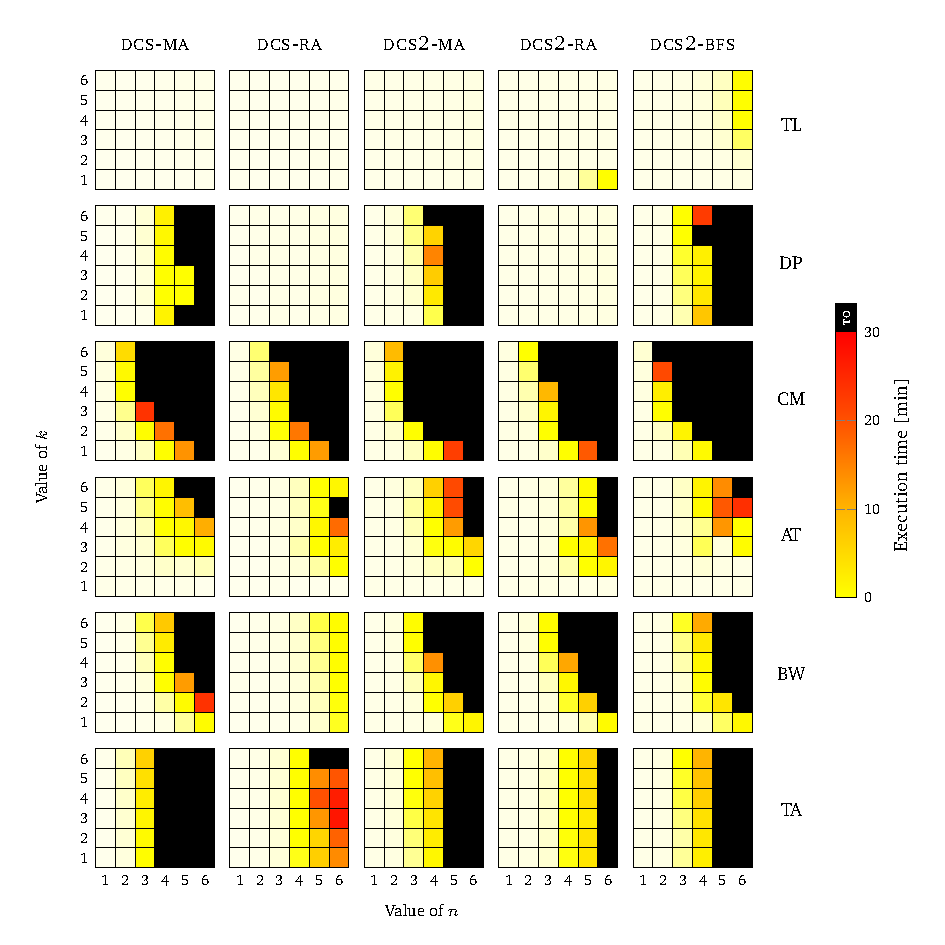
\includegraphics[width=\linewidth]{figures/benchmark/dcs_vs.pdf}\label{fig:dcs:results:detailed}
        \caption{\DCS detailed benchmark results.}
    \end{subfigure}%
    \begin{subfigure}{0.5\textwidth}
        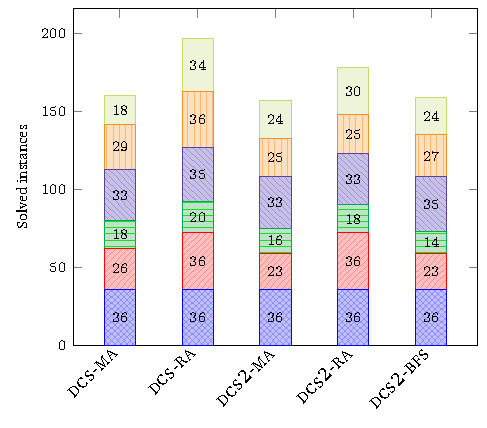
\includegraphics[width=0.9\linewidth]{figures/benchmark/dcs_instances.pdf}\label{fig:dcs:results:instances}
        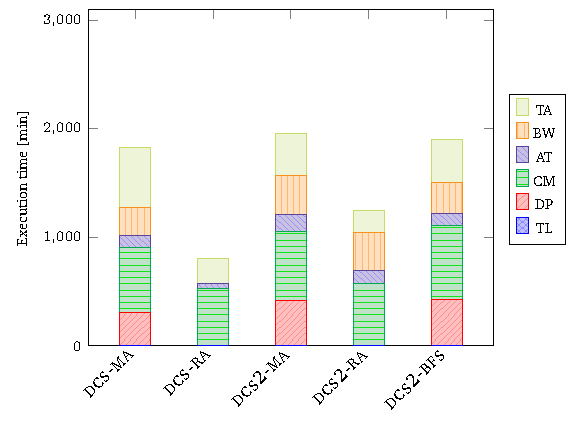
\includegraphics[width=\linewidth]{figures/benchmark/dcs_time.pdf}\label{fig:dcs:results:time}
        \caption{Total solved instances (top) and execution time (bottom) with \DCS.}
    \end{subfigure}
\caption{Benchmark results.}
\label{fig:dcs:results}
\end{figure}

En la figura~\ref{fig:dcs:results} se pueden observar los resultados con respecto a DCS anterior. Antes que nada podemos concluir que hay una ganancia al utilizar mejores heurísticas, ya que BFS pierde contra RA tanto en cantidad de instancias como tiempo. Sorprendentemente a pesar de ser muy naif termina compitiendo contra MA. Esto tiene su explicación en el cambio de objetivo, ya que MA fue presentada en \textcolor{red}{[REF reachability en paper]} para \textit{reachability}.

Nuestra versión (dcs2) mantiene la performance en la mayoría de los casos de estudio. En TA hay algunas instancias nuevas que dan timeout, pero el resto concluyen rápidamente. El único caso donde pierde notoriamente es BW, pero mirando otras herramientas (con la excepción de \MYND) vemos que en general tienen problemas con los casos más grandes de BW. Nuestra suposición es que la implementación DCS anterior clasificaba estados como $\Goals$ de manera anticipada y posiblemente erronea, quizás casos como el de \ref{test:goals:falsopositivo}. Esto puede hacer que se llegue a una conclusión apurada que posiblemente devuelva un controlador incorrecto, pero que en el benchmark parezca resolver más instancias.

\section{Comparación con otros programas}

Si bien nuestra exploración parece perder un poco de escalabilidad en ciertos casos, en la figura \ref{fig:tools:results} podemos ver que seguimos en una posición competitiva con respecto a otras herramientas del estado del arte. Para que sea más simple la comparación decidimos mostrar solo RA, ya que es la heurística de mejor desempeño, y ambas versiones de \DCS. 

Aunque la nueva versión esté un poco más lejos de \MYND, en calidad de cantidad de intancias y tiempo supera ampliamente el resto de las opciones, referirse a fig \ref{fig:tools:results:instances} y \ref{fig:tools:results:time}.
\begin{figure}[th]
    \centering
    \hspace*{-20mm}
    \begin{subfigure}{0.7\textwidth}
        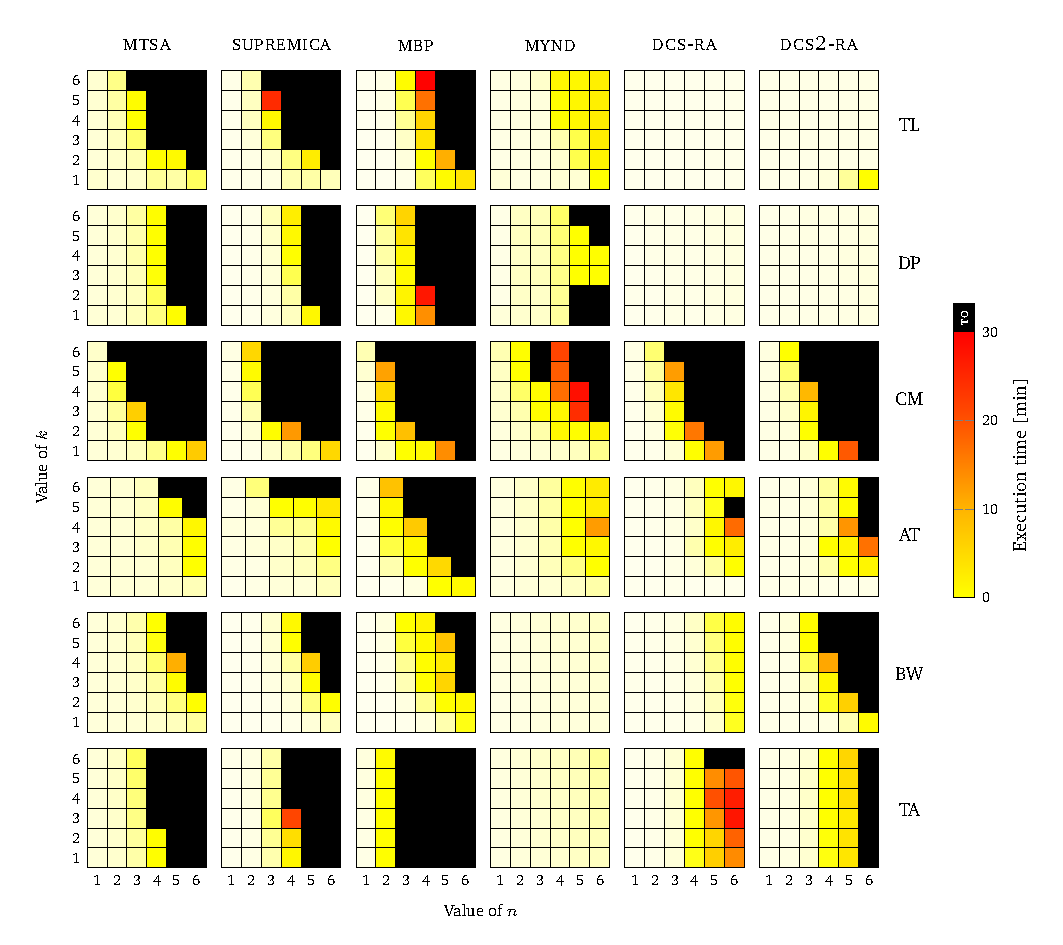
\includegraphics[width=\linewidth]{figures/benchmark/tools_vs.pdf}\label{fig:tools:results:detailed}
        \caption{\DCS detailed benchmark results.}
    \end{subfigure}%
    \begin{subfigure}{0.5\textwidth}
        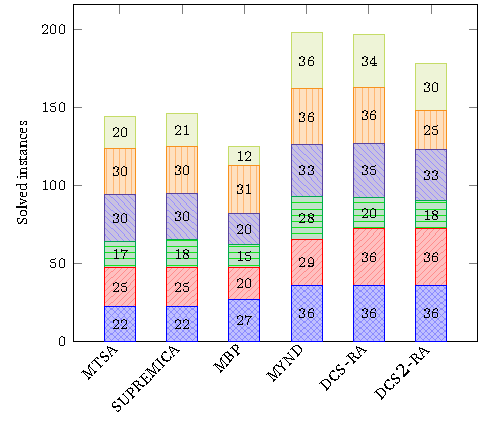
\includegraphics[width=0.9\linewidth]{figures/benchmark/tools_instances.pdf}\label{fig:tools:results:instances}
        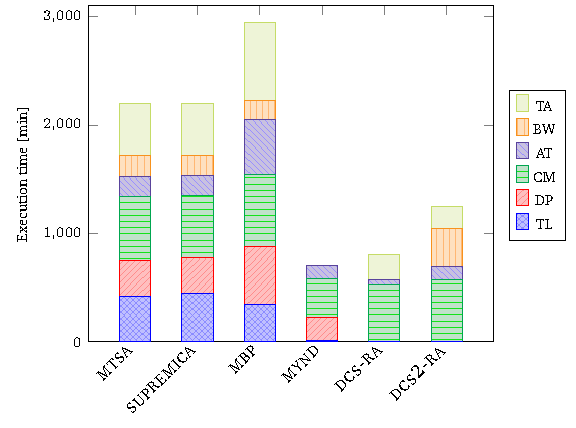
\includegraphics[width=\linewidth]{figures/benchmark/tools_time.pdf}\label{fig:tools:results:time}
        \caption{Total solved instances (top) and execution time (bottom) with \DCS.}
    \end{subfigure}
\caption{Benchmark results.}
\label{fig:tools:results}
\end{figure}


\chapter{Conclusiones}\label{chpt:conclusiones}
%- En conclusiones listaría los desafíos que tuvieron
% a) Entender el algoritmo de daniel
% b) Entender el algoritmo estandar
% c) Entender la implementación de daniel. Muy distinta. y el codigo de MTSA en general
% d) Entender control supervisado (composicional y no composicional)
% 
% y contribuciones:
% 
% 1) Tests de regression y harness que muestran los bugs
% 2) Nuevo algoritmo
% 3) Prueba
% 4) Experimentación mostrando que no hay perdida significativa de performance.

Al empezar con el proyecto y leer sobre control supervisado descubrimos que hay todo un mundo detrás. Primero debimos aprender sobre los algoritmos composicionales y no composicionales. Luego entender el algoritmo estándar y parte de su implementación para finalmente poder arrancar con el algoritmo on-the-fly. Éste último lo debimos entender a la perfección, para poder descubrir y solucionar los diversos problemas. 

MTSA es un proyecto con gran trayectoria y muchos avances en diversos frentes hechos por diferentes personas y grupos de investigación; como tal su código puede ser muy complejo, teniendo partes escritas incluso en versiones antiguas de java.\\

Pese a estos desafíos, logramos las siguientes contribuciones: 
\begin{itemize}
	\item Una batería de tests de regresión como una adición permanente al proyecto de MTSA para garantizar la continua correctitud de su feature de síntesis de controladores con exploración heurística.
	
	\item Un nuevo algoritmo de exploración, cuya correctitud es agnóstica a la heurística utilizada.
	
	\item Una prueba de la correctitud y completitud del algoritmo presentado.
	
	\item Resultados experimentales para comprobar que las modificaciones a la exploración siguen manteniendo la buena performance de la técnica.
\end{itemize}

%TODO TRABAJO A FUTURO
% casos de tests generados automáticamente por medio de mutaciones?


%%%% BIBLIOGRAFIA
\backmatter
\bibliography{biblio}

\end{document}
